% !TEX root = main.tex
\documentclass[conference]{IEEEtran}
\IEEEoverridecommandlockouts
% The preceding line is only needed to identify funding in the first footnote. If that is unneeded, please comment it out.
% \usepackage{fontspec}               % 加载 fontspec 包
% \usepackage{xeCJK}                    % 加载 xeCJK 包
% % \setCJKmainfont{WenQuanYi Zen Hei}  % 设置中文主字体
% \setCJKmainfont[Path=fonts/, Extension=.ttc]{wqy-zenhei}
% \usepackage{ulem}      % 删除线、normalem
\usepackage{hyperref}  % 超链接
% \usepackage{breakurl}
\usepackage{url}       % 处理参考文献中的下划线
\def\UrlBreaks{\do\A\do\B\do\C\do\D\do\E\do\F\do\G\do\H\do\I\do\J
\do\K\do\L\do\M\do\N\do\O\do\P\do\Q\do\R\do\S\do\T\do\U\do\V
\do\W\do\X\do\Y\do\Z\do\[\do\\\do\]\do\^\do\_\do\`\do\a\do\b
\do\c\do\d\do\e\do\f\do\g\do\h\do\i\do\j\do\k\do\l\do\m\do\n
\do\o\do\p\do\q\do\r\do\s\do\t\do\u\do\v\do\w\do\x\do\y\do\z
\do\.\do\@\do\\\do\/\do\!\do\_\do\|\do\;\do\>\do\]\do\)\do\,
\do\?\do\'\do+\do\=\do\#}
% \usepackage{cite}    % 与biblatex包冲突
\usepackage{amsmath,amssymb,amsfonts}
\usepackage{algorithm}
\usepackage{algorithmicx}
\usepackage{algpseudocode}
% \usepackage{multirow}  % 表格-合并单元格
% \usepackage{booktabs}  % 提供更美观的表格线
\usepackage{makecell}  % 提供加粗表格线的功能。
\renewcommand{\thefootnote}{\fnsymbol{footnote}}
\renewcommand{\algorithmicrequire}{\textbf{Input:}}
\renewcommand{\algorithmicensure}{\textbf{Output:}}
% \newcommand{\FUNCTION}[1]{\STATE \textbf{function} \textsc{#1}}
% \newcommand{\ENDFUNCTION}{\STATE \textbf{end function}}
\usepackage{graphicx}
\usepackage{textcomp}
\usepackage{xcolor}
\def\figTotalScene{\textwidth}
\def\figGradAscentAttack{0.5\textwidth}
\def\figLabelFlip{0.5\textwidth}
\def\figBackdoorAttack{0.5\textwidth}
\def\figGradAscentAttackDefense{0.5\textwidth}
\def\figLabelFlipDefense{0.5\textwidth}
\def\figBackdoorAttackDefense{0.5\textwidth}
% \usepackage{svg}
% \def\BibTeX{{\rm B\kern-.05em{\sc i\kern-.025em b}\kern-.08em
%     T\kern-.1667em\lower.7ex\hbox{E}\kern-.125emX}}

% \usepackage[style=ieee,backend=biber]{biblatex}
% \normalem  % 取消参考文献的下划线
% \addbibresource{references.bib}

% % 设置姓名缩写
% \AtBeginBibliography{%
%     \renewbibmacro*{bbx:savehash}{}%
%     \renewcommand*{\mkbibnamegiven}[1]{\uppercase{#1}}%
%     \renewcommand*{\mkbibnamefamily}[1]{\uppercase{#1}}%
% }
% % 替换下划线字符
% \DeclareSourcemap{
%     \maps[datatype=bibtex]{
%         \map{
%             \step[
%                 fieldsource=url,
%                 match=\regexp{_},
%                 replace=\regexp{\%5f}
%             ]
%         }
%     }
% }

\begin{document}

% 标题
\title{ViT-MGI: Context-aware Lightweight Malicious Gradient Identification for Federated Vision Transformer Systems against Poisoning Attacks\\
% {\footnotesize \textsuperscript{*}Note: Sub-titles are not captured in Xplore and
% should not be used}
% \thanks{Identify applicable funding agency here. If none, delete this.}
}

\author{

\IEEEauthorblockN{
    Shujie Yang\href{https://orcid.org/0000-0002-9597-2659}{
\includegraphics[width=8pt]{pics/orcid.png}}$^1$, 
    Tengfei Li\href{https://orcid.org/0000-0001-5412-8198}{
\includegraphics[width=8pt]{pics/orcid.png}}$^1$, 
    % Zan Zhou\href{https://orcid.org/0000-0003-2388-2280}{
\includegraphics[width=8pt]{pics/orcid.png}}$^1$\footnotemark[1], 
    Zan Zhou\href{https://orcid.org/0000-0003-2388-2280}{
\includegraphics[width=8pt]{pics/orcid.png}}$^1$\footnotemark\textsuperscript{\hyperref[fn:corresponding]{*}},
    Su Yao\href{https://orcid.org/0000-0001-5165-2787}{
\includegraphics[width=8pt]{pics/orcid.png}}$^2$, 
    Tianyu Xu\href{https://orcid.org/0009-0001-5694-476X}{
\includegraphics[width=8pt]{pics/orcid.png}}$^1$,
    Bo Wang\href{https://orcid.org/0009-0004-7889-5390}{
\includegraphics[width=8pt]{pics/orcid.png}}$^1$
}
\IEEEauthorblockA{\textit{$^1$School of Computer Science, Beijing University of Posts and Telecommunications, Beijing, China}\\
\textit{$^2$Beijing National Research Center for Information Science and Technology, Tsinghua University, Beijing, China}
}

% \and

% \IEEEauthorblockN{1\textsuperscript{st} Shujie Yang}
% \IEEEauthorblockA{\textit{School of Computer Science} \\
% \textit{BUPT}\\
% Beijing, China \\
% \href{https://orcid.org/0000-0002-9597-2659}{0000-0002-9597-2659
\includegraphics[width=8pt]{pics/orcid.png}}}
% \and
% \IEEEauthorblockN{2\textsuperscript{nd} Given Name Surname}
% \IEEEauthorblockA{\textit{dept. name of organization (of Aff.)} \\
% \textit{name of organization (of Aff.)}\\
% City, Country \\
% email address or ORCID}
% \and
% \IEEEauthorblockN{3\textsuperscript{rd} Given Name Surname}
% \IEEEauthorblockA{\textit{dept. name of organization (of Aff.)} \\
% \textit{name of organization (of Aff.)}\\
% City, Country \\
% email address or ORCID}
% \and
% \IEEEauthorblockN{4\textsuperscript{th} Given Name Surname}
% \IEEEauthorblockA{\textit{dept. name of organization (of Aff.)} \\
% \textit{name of organization (of Aff.)}\\
% City, Country \\
% email address or ORCID}
% \and
% \IEEEauthorblockN{5\textsuperscript{th} Given Name Surname}
% \IEEEauthorblockA{\textit{dept. name of organization (of Aff.)} \\
% \textit{name of organization (of Aff.)}\\
% City, Country \\
% email address or ORCID}
% \and
% \IEEEauthorblockN{6\textsuperscript{th} Given Name Surname}
% \IEEEauthorblockA{\textit{dept. name of organization (of Aff.)} \\
% \textit{name of organization (of Aff.)}\\
% City, Country \\
% email address or ORCID}

}

\maketitle

% \footnotetext[1]{Corresponding author. Email: zan.zhou@example.com}
\footnotetext[1]{Corresponding author:\label{fn:corresponding} \href{mailto:zan.zhou@bupt.edu.cn}{zan.zhou@bupt.edu.cn}}

% 摘要
\begin{abstract}

% 联邦学习可以在数据不离开客户端的前提下进行模型训练,保护了用户的隐私且减小了中央服务器的压力。然而,在联邦学习的过程中,经常会有恶意客户端的存在。当然,恶意用户的数量一般会占据较小的部分。本文对联邦学习过程中用户上传上来的梯度变化进行分析,首先利用最大池化技术提取主要特征的同时降低,利用主成分分析(PCA)算法\textcolor{red}{(这里还有待添加更多的算法)}对恶意用户进行识别。单次被识别为恶意用户可能是由于误判,因此本文使用主观逻辑模型来对用户的信用等级进行评估,并依据用户的可信度来调整模型聚合时的权重。

% 结果表明,当前方法对于恶意用户的识别率、恶意用户的识别效率,以及程序自身的鲁棒性都有所提升。我们将其命名为FLDefinder\textcolor{red}{(名字待定)}并发布了其源代码,以方便该领域的未来研究:\href{https://github.com/LetMeFly666/FLDefinder}{https://github.com/LetMeFly666/FLDefinder}\textcolor{red}{(论文投稿前此仓库为Private状态不可访问)}。

% 随着视觉大模型的不断发展,模型训练时需要越来越大的数据量。因此需要联邦学习的ViT模型(Federated ViT),在数据不离开多个客户端的前提下进行模型训练,同时捕捉复杂的全局特征\footnote{相比于简单的CNN等,ViT可以更好地捕捉全局信息}。例如FeSTA通过分割学习的ViT模型进行COVID-19的胸部X光片检测,保留数据隐私的同时在多个数据集上实现了性能提升\cite{federatedViT_example}。然而,在实际的应用场景中,各式各样的攻击对联邦学习带来了很大的问题。例如,有的攻击者会篡改本地训练出的梯度数据,从而扰乱聚合后的全局模型的效果;有的攻击者会篡改数据集的标签,例如常见的标签翻转,来诱导模型对特定事物造成错误的判断\cite{tailAttack_SuchAsLabelFlip};还有的攻击者会采用更加隐蔽的后门攻击,在训练过程中设计难以被识别的触发器从而达到插入后门的效果\cite{backdoor_001}。

% With the continuous development of large vision models, model training requires increasingly large datasets. Therefore, Federated Learning for Vision Transformer models (Federated ViT) is needed to train models without data leaving multiple clients, while capturing complex global features. For example, FeSTA uses a Federated ViT model for COVID-19 chest X-ray detection, enhancing performance across multiple datasets while preserving data privacy\cite{federatedViT_example}. However, in practical applications, various attacks pose significant challenges to federated learning. For instance, some attackers may tamper with locally trained gradient data, thereby disrupting the effectiveness of the aggregated global model; some attackers may alter dataset labels, such as the common label-flipping attack, to mislead the model into making incorrect judgments on specific matters\cite{tailAttack_SuchAsLabelFlip}; and others may employ more covert backdoor attacks, designing triggers during training that are difficult to detect, thus achieving the insertion of backdoors\cite{backdoor_001}.

% % 针对这些攻击,已有多种防御机制被提出,包括Krum算法、multi-Krum算法\cite{aggregation_Krum}、中值算法、裁剪平均算法\cite{aggregation_MedianTrimmedMean}、Principal Component Analysis(PCA)\cite{federatedPCA}和Sniper方案\cite{aggregation_Sniper}等。这些方法在一定程度上能解决恶意用户的攻击问题,但在Federated ViT场景下普遍存在效率低、鲁棒性差的缺陷。ViT模型的参数量巨大,导致现有防御方案在处理ViT场景下的恶意攻击时耗时显著增加。此外,ViT模型中大量不活跃的神经元在恶意用户和正常用户之间差异不明显,从而降低了检测效率和鲁棒性。

% To counter these attacks, various defense mechanisms have been proposed, including the Krum algorithm, multi-Krum algorithm\cite{aggregation_Krum}, median algorithm, trimmed mean algorithm\cite{aggregation_MedianTrimmedMean}, Principal Component Analysis (PCA)\cite{federatedPCA}, and the Sniper scheme\cite{aggregation_Sniper}. These methods can partially address malicious user attacks, but they generally exhibit low efficiency and poor robustness in Federated ViT scenarios. The vast number of parameters in ViT models leads to significantly increased processing time for existing defense schemes when dealing with malicious attacks in ViT contexts. Furthermore, the large number of inactive neurons in ViT models show minimal differences between malicious and benign users, thereby reducing detection efficiency and robustness.

% % In this paper,我们提出了一种针对ViT的两阶段的上下文感知轻量级恶意梯度识别方法来提升检测恶意用户的效率和鲁棒性。我们通过特征层提取和主成分分析算法(PCA)去除无效的梯度信息,从而在提升检测效率的同时提升了检测的鲁棒性。Specifically,对于用户上传上来的梯度信息,模型首先进行特征层提取,保留有效信息的同时降低数据维度。接着使用PCA算法对数据进行再次降维。两次降维之后,我们成功在不降低检测准确率的情况下将数据维度下降到原来的0.4\%。随后我们使用隔离森林算法依据提取出的梯度特征鉴别恶意用户和良性用户。最后,我们使用主观逻辑模型\cite{Subjective_Logic_Model}进行时域累计的用户评分并在聚合梯度信息的过程中加以考虑,这样使得判断结果更好的同时减少了由于随机森林的随机性而导致的错误判定\footnote{因为多次都错误封禁一个恶意用户的概率会指数级别的减小}。这样,在ViT这种具有大量参数的模型下,我们的模型也能够进行很好的联邦学习训练并杜绝可能的潜在的攻击。

% In this paper, we propose a two-stage, context-aware lightweight malicious gradient identification method specifically for ViT to improve the efficiency and robustness of malicious user detection. By using feature layer extraction and Principal Component Analysis, we eliminate invalid gradient information, thereby enhancing both detection efficiency and robustness. Specifically, for the gradient information uploaded by users, the model first performs feature layer extraction to retain useful information while reducing data dimensions. Then, PCA is used to further reduce the dimensions. After these two stages of dimensionality reduction, we successfully reduced the data dimensions to 0.4\% of the original without compromising detection accuracy. Next, we use the Isolation Forest algorithm to distinguish between malicious and benign users based on the extracted gradient features. Finally, we employ a Subjective Logic Model\cite{Subjective_Logic_Model} to perform temporal accumulation of user scores and consider these scores during gradient aggregation. This approach not only improves the accuracy of judgments but also reduces erroneous identifications caused by the randomness of the Isolation Forest. Thus, even with the large number of parameters in ViT models, our method ensures effective federated learning training and mitigates potential attacks.

% % 我们在CIFAR-10、MNIST、OrganAMNIST等数据集上做了有关模型效率以及有关识别鲁棒性的实验,结果显示在处理时间上,我们的模型比先进的PCA方法降低了大约70\%。此外模型在准确率和F1分数上较PCA方法都有较大提升。同时,我们对比了池化技术来减少计算量并增强鲁棒性的算法,结果显示,相较于池化方法,我们的方法在效率和鲁棒性方面均有较大优势\cite{betterTogether}。

% % 我们将模型命名为ViT-MGI并发布了其源代码,以方便该领域的未来研究:\href{https://github.com/LetMeFly666/FLDefinder}{https://github.com/LetMeFly666/FLDefinder}\footnote{论文投稿前此仓库为Private状态不可访问}。

% We conducted experiments on datasets such as CIFAR-10, MNIST, and OrganAMNIST to evaluate the efficiency and robustness of our model. The results show that our model reduces processing time by approximately 70\% compared to the advanced PCA method. Moreover, our model significantly improves accuracy and F1 scores compared to the PCA method. Additionally, we compared pooling techniques aimed at reducing computational load and enhancing robustness. The results indicate that our method offers substantial advantages in both efficiency and robustness compared to pooling methods\cite{betterTogether}.

With the continuous development of large vision models, training requires increasingly large datasets. Federated Learning for Vision Transformer models (Federated ViT) is needed to train models without data leaving multiple clients while capturing complex global features. However, various attacks, such as tampering with gradient data, label-flipping, and backdoor attacks, pose significant challenges to federated learning. Existing defense mechanisms like the Krum algorithm, PCA, and Sniper scheme exhibit low efficiency and poor robustness in Federated ViT scenarios due to the vast number of parameters and inactive neurons.

This paper proposes a two-stage, context-aware lightweight malicious gradient identification method for ViT to improve the efficiency and robustness of malicious user detection. By using feature layer extraction and Principal Component Analysis (PCA), we eliminate invalid gradient information, enhancing both detection efficiency and robustness. We reduced data dimensions to 0.4\% of the original without compromising detection accuracy. The Isolation Forest algorithm distinguishes between malicious and benign users based on extracted gradient features, and a Subjective Logic Model performs temporal accumulation of user scores to improve accuracy and reduce erroneous identifications.

Experiments on CIFAR-10, MNIST, and OrganAMNIST datasets show that our model reduces processing time by approximately 70\% compared to advanced PCA methods, while significantly improving accuracy and F1 scores. Additionally, our method offers substantial advantages in both efficiency and robustness compared to pooling techniques aimed at reducing computational load.

We have named our model ViT-MGI and released its source code to facilitate future research in this field: \href{https://github.com/LetMeFly666/FLDefinder}{https://github.com/LetMeFly666/FLDefinder}.

% 下面是关于摘要的大纲

% Abstract:

% 随着视觉大模型的发展,训练需要更多数据量,所以要做Fedteratred ViT。(可举例)

% 但是这里面会存在恶意攻击者污染xx(待扩展,比如xx攻击 实际例子也可)。

% (问题)现有很多防御也提出了xx(不用太多)。However存在(安全效率冲突)问题。(可解释:)更复杂、数据更离散...   导致了现有防御方案在Fedteratred ViT下针对它们的防御存在效率低(xx模型参数多少 耗时要提高xx倍 )下,不鲁棒xxx缺陷(可举例) 。(比如一下xxxx万参数,我xx的池化限制到xx,(和CNN差不多))

% (方法) In this paper,我们提出了一种两阶段的xx方法来提升效率、鲁棒性,通过xx理念解决xx问题(一句话:核心思想)。具体来说Specifically,首先通过xxx来xx了xx\%,随后我们xxx,最终/从而 实现了xx(具体是xx方法,别虚话)。

% (效果)我们在多少数据集上做了多少实验,从xx方面显示我们比xx等(当前最新)防御方法取得了xx提升。(若实验很好可多写点:在效率上提升了xx倍,在精度上xx  (详述))

\end{abstract}


\begin{IEEEkeywords}

Federated Learning, Gradient Analysis, Malicious User Detection, Subjective Logic Model, Feature Layer Extraction
\end{IEEEkeywords}

\section{Introduction}

\label{sec:intro}

% 联邦学习(FL)使参与者能够联合训练一个全局模型,而不需要共享他们的数据集\cite{FLGenesisArticle, BetterTogether29}。

% \textcolor{red}{上一段其实是抄的BetterTogether}

% % 如今,边缘设备的激增使得数据量爆炸式增长\cite{edgeComputing_explosiveGrowth},数据隐私的重要性也正显得越来越重要。2024年,全球大约75\%的人口将受到现代隐私法规的保护。这些法规的扩展推动了隐私实践的实施,并且大型企业在数据隐私方面的年均预算预计将超过250万美元\cite{dataPrivacyIsEncreasing}。为了解决这一问题,一种越来越流行的方式是使用联邦学习\cite{useFL2solve}。联邦学习(Federated Learning, FL)是一种分布式机器学习方法,旨在在多个分散的数据源上进行协作训练,同时避免将数据集中存储。FL由McMahan等人于2016年提出,通过在客户端设备上进行本地模型训练,并仅上传模型更新到中央服务器进行聚合,从而保护数据隐私和安全。一旦聚合,服务器将更新后的模型广播回所有客户端。节点将在本地更新其模型,并使用更新后的模型与新一批本地数据进行下一轮本地训练。这种方法不仅减少了数据传输的需求,还能在不暴露原始数据的情况下,利用分散的数据源提高模型性能\cite{FLGenesisArticle}\footnote{这段Intro参考Mitigating Adversarial写的}。

% The surge in edge devices has led to an explosive growth in data volume\cite{edgeComputing_explosiveGrowth}, making data privacy increasingly important. By 2024, approximately 75\% of the global population will be protected by modern privacy regulations. These regulations are driving the implementation of privacy practices, with large companies expected to allocate over \$2.5 million annually to data privacy\cite{dataPrivacyIsEncreasing}. To address this issue, an increasingly popular approach is the use of Federated Learning (FL)\cite{useFL2solve}. Federated Learning is a distributed machine learning method designed to collaboratively train models across multiple decentralized data sources while avoiding centralized data storage. Proposed by McMahan et al. in 2016, FL involves local model training on client devices, with only the model updates being uploaded to a central server for aggregation, thereby safeguarding data privacy and security. Once aggregated, the server broadcasts the updated model back to all clients. The clients then update their local models and use the updated model with a new batch of local data for the next round of training. This approach not only reduces the need for data transmission but also leverages decentralized data sources to improve model performance without exposing the original data\cite{FLGenesisArticle}.

% % 联邦学习中一个流行的训练模型是Transformer\cite{transformer},Transformer模型引入了自注意力机制(self-attention mechanism),能够在处理输入序列时捕捉长距离依赖关系,从而显著提高了模型的性能和并行处理能力,并且能够有效地被运用在翻译\cite{transformer_translation}、音频分类\cite{transformer_audioClassification}、计算机视觉(ViT)\cite{transformer_vision}等多个领域。联邦学习中对ViT进行训练或微调引起了业界和学术界的广泛兴趣\cite{transformer_gotInterest},该系列模型需要大量的设计以及强大的计算资源,因此在训练过程中需要特别注意保护模型的完整性。\footnote{这段Intro参考Mitigating Adversarial写的}

% A popular training model in federated learning is the Transformer\cite{transformer}, which introduces the self-attention mechanism. This mechanism captures long-range dependencies when processing input sequences, significantly enhancing the model's performance and parallel processing capabilities. The Transformer model has been effectively applied in various fields, including translation\cite{transformer_translation}, audio classification\cite{transformer_audioClassification}, and computer vision (Vision Transformer)\cite{transformer_vision}. Training or fine-tuning ViT models in federated learning has garnered extensive interest from both industry and academia\cite{transformer_gotInterest}. These models require extensive design and powerful computational resources, making it crucial to ensure the integrity of the model during the training process.

% % Suppose there are some malicious clients,在客户端向服务器发送训练得到的梯度之前,首先对梯度进行更改,例如对梯度取反,从而严重破环全局模型的训练质量。或者会存在一些恶意客户端,篡改本地数据,诱导中央服务器学到一些错误特征从而达到植入后门的效果。这些行为都会严重影响最终的训练结果,甚至会造成一些安全性的问题。

% Suppose there are some malicious clients. Before sending the locally trained gradients to the server, these clients alter the gradients, such as by reversing their values, thereby severely compromising the training quality of the global model. Additionally, some malicious clients might tamper with local data to mislead the central server into learning incorrect features, effectively inserting a backdoor into the model. These actions can significantly impact the final training results and potentially introduce serious security issues.

% % 针对这些攻击,现已提出了很多防御机制,有通过在服务器上计算每个模型更新与其最近更新之间的欧氏距离之和来决定是否聚合模型更新的Krum算法和拓展的multi-Krum算法\cite{aggregation_Krum},有选择中值或排除边缘值后的平均值作为全局模型的中值算法和裁剪平均算法\cite{aggregation_MedianTrimmedMean},也有使用主成分分析(Principal Component Analysis, PCA)来检测恶意用户的算法\cite{federatedPCA},以及通过解决最大团问题(Maximum CliqueProblem, MCP)从而无需恶意用户数量这一先验知识的Sniper方案\cite{aggregation_Sniper}。这些数据都能在不同程度上解决恶意用户的攻击问题,但在Fedteratred ViT场景下这些方法普遍存在效率低、鲁棒性差等缺陷。原因在于很小的ViT-B/16模型也有千万级别的参数,相比于参数级别为百万甚至十万的传统CNN模型,即使是线性复杂度的安全检测方法,在处理Vit场景下的恶意攻击的耗时也要提升几十倍甚至几百倍\footnote{这一句在说参数量大所以原有防御方案效率低}。我们注意到在庞大的ViT模型中,存在大量不活跃的神经元,这些神经元在恶意用户和正常用户之间的差异不明显,从而降低了恶意攻击检测的效率和鲁棒性。\footnote{这一句在说参数散多所以原有防御方案鲁棒性差}。

% To counter these attacks, many defense mechanisms have been proposed. The Krum algorithm and its extension, the multi-Krum algorithm\cite{aggregation_Krum}, calculate the sum of Euclidean distances between each model update and its nearest updates to decide whether to aggregate the model updates. The median algorithm and trimmed mean algorithm select the median or the mean after excluding outliers as the global model\cite{aggregation_MedianTrimmedMean}. Principal Component Analysis has also been used to detect malicious users\cite{federatedPCA}, and the Sniper scheme addresses the problem by solving the Maximum Clique Problem\cite{aggregation_Sniper}, which does not require prior knowledge of the number of malicious users. While these methods can address malicious user attacks to varying degrees, they generally suffer from low efficiency and poor robustness in Federated ViT scenarios. The reason is that even a small ViT-B/16 model has tens of millions of parameters, compared to the millions or hundreds of thousands of parameters in traditional CNN models. Even security detection methods with linear complexity require dozens to hundreds of times more processing time when dealing with malicious attacks in ViT scenarios. We observe that in large ViT models, there are many inactive neurons whose differences between malicious and benign users are not apparent, reducing the efficiency and robustness of malicious attack detection.

% % In this work,我们专注于对针对恶意用户上传恶意梯度从而攻击服务器模型的行为进行系统的防御。图\hyperref[fig:totalScene]{\ref{fig:totalScene}}描述了在正常训练中存在梯度上升攻击的恶意用户的情况。图的下方是参与训练的客户端,它们首先接收中央服务器广播下发的全局模型,然后使用本地数据对模型进行一定量的训练,之后再将训练得到的梯度变化汇总到中央服务器上,从而完成一轮总的训练。假设在参与训练的客户端中出现了一些恶意用户(如图\hyperref[fig:totalScene]{\ref{fig:totalScene}}中的ViT-I),它们出于一定的目的想要干扰中央服务器的模型训练结果。于是它们在将训练得到的梯度变化上传到中央服务器之前,先对这些梯度进行一些修改操作,例如将梯度取反等,从而试图下降总模型的训练效果。

% In this work, we focus on systematically defending against behaviors where malicious users upload malicious gradients to attack the server model. Figure \hyperref[fig:totalScene]{\ref{fig:totalScene}} illustrates the scenario where malicious users perform gradient ascent attacks during normal training. The bottom part of the figure shows the participating clients, which first receive the global model broadcasted by the central server, then train the model using their local data, and finally upload the resulting gradient changes back to the central server to complete one round of training. Suppose some malicious users are among the participating clients (e.g., ViT-I in Figure \hyperref[fig:totalScene]{\ref{fig:totalScene}}). They aim to disrupt the central server's model training. Before uploading the locally trained gradients, they modify these gradients, such as reversing them, in an attempt to degrade the overall model's training performance.

% % In this Paper,我们提出了ViT-MGI:对于如图所示的恶意用户的攻击行为,ViT-MGT是一种有效的防御手段。它首先对模型上传上来的梯度进行特征层提取和主成分分析操作,减少后续识别所需数据量的同时,成功剔除了大量无效的信息。这些“无效”信息是由于ViT模型的体积较大所导致的,对于单次训练,大量(例如ViT-B/16具有86百万级别的参数量)的梯度变化中,有很多梯度的变化几乎为0。如果不进行降维操作,这些对于攻击识别几乎无效的大量数据不仅会增加后续计算的复杂度,还会增加攻击者和正常参与者梯度之间的相似程度。在进行主成分分析以及后续的识别时,我们只关注ViT模型中一些对于攻击比较敏感的层,因为我们通过实验\hyperref[exp:exp_layer]{\ref{exp:exp_layer}}得知,存在梯度上升、标签翻转、后门植入等常见的甚至未知的攻击时,这些层的变化最为敏感,而其他层变化普遍较小,甚至几乎为0。经过降维处理后就只剩下敏感的少量的权重变化了。最后,使用异常检测手段例如隔离森林,就能轻松准确地识别出恶意攻击的存在。考虑到实际训练过程中可能会存在很多随机因素,因此可能会出现一定的错误识别现象,即一些正常用户的梯度偶尔可能会和恶意用户较为相似,从而导致此轮次被错误识别为恶意行为用户,我们使用主观逻辑模型来对每个用户评分并在聚合梯度信息的过程中加以考虑,显著减少了由于随机因素导致的错误封禁。

% In this paper, we propose ViT-MGI: an effective defense mechanism against the malicious user attacks depicted in the figure\hyperref[fig:totalScene]{\ref{fig:totalScene}}. ViT-MGI first performs feature layer extraction and principal component analysis on the gradients uploaded by the model. This reduces the amount of data needed for subsequent identification while successfully eliminating a large amount of redundant information. These "redundant" pieces of information arise due to the large size of the ViT model. For instance, in a single training instance, a vast number of gradient changes (e.g., the ViT-B/16 model has 86 million parameters) are nearly zero. Without dimensionality reduction, these largely ineffective data points for attack detection not only increase the complexity of subsequent computations but also heighten the similarity between the gradients of attackers and legitimate participants.

% During PCA and subsequent identification, we focus only on layers of the ViT model that are particularly sensitive to attacks. Our experiments \hyperref[exp:exp_layer]{\ref{exp:exp_layer}} show that these layers exhibit the most significant changes under common and even unknown attacks, such as gradient ascent, label flipping, and backdoor insertion, while other layers exhibit minimal or almost zero changes. After dimensionality reduction, only a small number of sensitive weight changes remain. Finally, we employ anomaly detection methods, such as Isolation Forest, to accurately identify the presence of malicious attacks.

% Given that random factors might exist during actual training, leading to some instances where normal users' gradients occasionally resemble those of malicious users, we use a subjective logic model to score each user. This scoring is considered during gradient aggregation, significantly reducing the likelihood of false bans due to random factors.

The surge in edge devices has led to explosive data growth, making data privacy increasingly important\cite{edgeComputing_explosiveGrowth}. By 2024, approximately 75\% of the global population will be protected by modern privacy regulations, driving large companies to allocate significant resources to data privacy. Federated Learning (FL) addresses this issue by enabling collaborative model training across decentralized data sources while avoiding centralized data storage\cite{useFL2solve}. Proposed by McMahan et al. in 2016, FL involves local model training on client devices, with only model updates uploaded to a central server for aggregation, thus safeguarding data privacy\cite{FLGenesisArticle}.

A popular training model in FL is the Transformer, which introduces the self-attention mechanism to capture long-range dependencies, significantly enhancing performance and parallel processing capabilities\cite{transformer}. The Vision Transformer (ViT) has been effectively applied in various fields, including translation\cite{transformer_translation}, audio classification\cite{transformer_audioClassification}, and computer vision\cite{transformer_vision}. Training ViT models in FL is of great interest to both industry and academia\cite{transformer_gotInterest}, requiring extensive design and computational resources to ensure model integrity.

However, malicious clients can significantly compromise the global model by tampering with locally trained gradients or altering local data to mislead the central server. These actions introduce security issues and degrade training quality. To counter such attacks, various defense mechanisms have been proposed, including the Krum algorithm, PCA, and Sniper scheme\cite{aggregation_Krum, aggregation_MedianTrimmedMean, federatedPCA, aggregation_Sniper}. These methods, however, exhibit low efficiency and robustness in Federated ViT scenarios due to the large number of parameters and inactive neurons in ViT models.

This paper proposes ViT-MGI, a two-stage, context-aware lightweight malicious gradient identification method to improve the efficiency and robustness of malicious user detection in ViT. ViT-MGI uses feature layer extraction and PCA to eliminate invalid gradient information, enhancing detection efficiency and robustness. Experiments show that our model reduces data dimensions to 0.4\% of the original without compromising detection accuracy. The Isolation Forest algorithm distinguishes between malicious and benign users based on extracted gradient features, and a Subjective Logic Model performs temporal accumulation of user scores to improve accuracy and reduce erroneous identifications. This approach ensures effective federated learning training and mitigates potential attacks, even with the large number of parameters in ViT models.

Our experiments on CIFAR-10, MNIST, and OrganAMNIST datasets demonstrate that ViT-MGI reduces processing time by approximately 70\% compared to advanced PCA methods while significantly improving accuracy and F1 scores. This method also offers substantial advantages in both efficiency and robustness compared to pooling techniques aimed at reducing computational load.

Our main contributions are as follows:

% \begin{enumerate}
%     \item 我们证明,在针对ViT这种体积较大的模型时,可以使用特征层提取的方式来降低数据维度并提升恶意梯度的识别效率。
%     \item 我们的ViT-MGI能够结合多轮训练结果跟随并感知恶意用户的行为,从而提升了整体的鲁棒性,具有较高的检测准确率,在多种攻击下都能在较低轮次以内区分出恶意客户端和正常用户。
%     \item 我们的ViT-MGI能够在较高的效率下完成恶意客户端的识别。
%     \item 我们能够在多达$30\%$攻击者进行不明显攻击时有效识别恶意攻击者。
%     \item 我们设计了一系列巧妙的实验证明了ViT-MGI的有效性。
% \end{enumerate}

\begin{enumerate}
    \item We demonstrate that for large-scale models like ViT, the use of feature layer extraction can effectively reduce data dimensionality and improve the efficiency of malicious gradient identification.
    \item Our ViT-MGI can track and detect the behaviors of malicious users over multiple training rounds, thereby enhancing overall robustness. It achieves high detection accuracy and can distinguish between malicious clients and normal users within a few rounds under various attack scenarios.
    \item ViT-MGI can efficiently identify malicious clients.
    \item We can effectively identify malicious attackers even when up to 30\% of the attackers perform subtle attacks.
    \item We have designed a series of ingenious experiments to prove the effectiveness of ViT-MGI.
\end{enumerate}

The rest of the paper is as follows. \hyperref[sec:related]{§\ref{sec:related}}surveys related work. \hyperref[sec:model]{§\ref{sec:model}} presents our system model. \hyperref[sec:method]{§\ref{sec:method}} describes the principles of the ViT-MGI shielding defense. We evaluate it on ViT-B/16 against a gradient-based attack and discuss the results in \hyperref[sec:exp]{§\ref{sec:exp}}. Finally, we conclude in \hyperref[sec:conclusion]{§\ref{sec:conclusion}}.

% Introduction:

% (创新点:核心-效率、精度-跟随-感知、实验)

% 列几点(至少上面的3点):

% \begin{enumerate}
%     \item ssf
%     \item sfs
% \end{enumerate}

% 一段话的本文结论 第二章是xx,section 3是xxx。(可参考IEEE transction)

\section{Related Work}
\label{sec:related}

% 在联邦学习对抗性攻击的投毒攻击中,通常有梯度上升攻击\cite{gradientAscentAttack}\footnote{检索关键词:"Gradient ascent attack" AND "Federated learning"}、假标签攻击\cite{fakeLabelAttack}\footnote{检索关键词:"fake label" AND "Federated learning"}以及后门攻击\cite{how2backdoor}这几类。其中,梯度上升或梯度扰乱攻击,以及假标签攻击都属于拜占庭攻击。

In federated learning, poisoning attacks typically include gradient ascent attacks\cite{gradientAscentAttack}, fake label attacks\cite{fakeLabelAttack}, and backdoor attacks\cite{how2backdoor}. Among these, gradient ascent or gradient perturbation attacks and fake label attacks are categorized as Byzantine attacks.

% 拜占庭攻击:攻击者试图破坏训练可用性和模型可用性,使其无法收敛或无法在主要训练任务中达到最优性能,并且不针对任何特定的用户或数据样本。其中,梯度上升攻击是指攻击者在本地训练时,将梯度上升方向的信息反转,从而在全局模型聚合时对全局模型造成破坏\cite{gradientAscentAttack}。针对这种攻击,G Lu等人提出了DEFEAT框架\cite{gradientAscentAttack_privacy},通过依赖对等网络(P2P)在客户端之间传递模型参数,避免了中央服务器的集中管理,但是其主要目的是防止梯度泄露的隐私问题。A. Grammenos等人使用主成分分析算法增强联邦学习的安全性\cite{federatedPCA},但其是一种差分隐私算法。假标签攻击又分为脏标签攻击(Dirty-labelAttack)\cite{latentAttack}和清洁标签攻击(Clean-labelAttack)\cite{cleanLabelAttack}。脏标签攻击会篡改数据集的标签,如常见的标签翻转攻击\cite{tailAttack_SuchAsLabelFlip},而清洁标签攻击不篡改标签,仅对数据进行处理生成新的样本。Lewis等人提出了Viceroy算法\cite{gradientAscentAttackAndLabelFlip},通过实施安全多方计算(Secure Multi-Party Computation, MPC)和差分隐私(Differential Privacy, DP)来检测并抵抗拜占庭攻击并提高系统隐私安全性。其文章中也指出,现有联邦学习防御系统在面对复杂和持续的梯度上升攻击时,通常会表现出鲁棒性不足的问题。并且Viceroy算法在面对ViT这种复杂度较高的模型时会暴露出通信开销较大和检测复杂度上升的问题。

Byzantine attacks involve adversaries attempting to disrupt the usability of the training process and the effectiveness of the model, preventing it from converging or achieving optimal performance in the primary training task without targeting any specific user or data sample. Gradient ascent attacks are a type of Byzantine attack where adversaries reverse the gradient ascent direction during local training, thereby damaging the global model during aggregation\cite{gradientAscentAttack}. To counter this attack, G. Lu et al. proposed the DEFEAT framework\cite{gradientAscentAttack_privacy}, which relies on peer-to-peer networks for transmitting model parameters between clients, thus avoiding centralized server management. However, its primary purpose is to prevent gradient leakage for privacy protection. A. Grammenos et al. employed principal component analysis to enhance federated learning security\cite{federatedPCA}, though this approach is essentially a differential privacy algorithm. Fake label attacks can be further divided into dirty-label attacks\cite{latentAttack} and clean-label attacks\cite{cleanLabelAttack}. Dirty-label attacks involve tampering with the dataset labels, such as through label flipping\cite{tailAttack_SuchAsLabelFlip}, whereas clean-label attacks process the data to generate new samples without altering the labels. Lewis et al. introduced the Viceroy algorithm\cite{gradientAscentAttackAndLabelFlip}, which employs secure multi-party computation and differential privacy to detect and resist Byzantine attacks, thereby enhancing system privacy and security. Their study also pointed out that existing federated learning defense systems generally lack robustness when facing complex and sustained gradient ascent attacks. Furthermore, the Viceroy algorithm exhibits significant communication overhead and increased detection complexity when dealing with highly complex models like ViT.

% 后门攻击:又叫木马攻击(Trojan Attack),攻击者试图使模型在某些目标任务上实现特定表现,同时保持模型在主要任务上保持良好的性能\cite{canYouBackdoor}。不同于主要目标是降低主任务总体性能的拜占庭攻击,后门攻击的目的通常是未知的,因此通常更难被检测。X. Gong等人对现有的backdoor攻击及防御手段做了系统的分析,指出了联邦学习框架下后门攻击和防御的各种潜在未来方向\cite{backdoorAndDefense}。C. Xie等人提出了专门针对backdoor的Certifiably Robust Federated Learning(CRFL)模型,他们exploited clipping and smoothing on model parameters to control the global model smoothness,从而对有限幅度的后门产生样本稳健性认证\cite{backdoorAndDefense_robust}。这在一定程度上取得了不错的效果,但其实际的计算开销较大。S. Andreina等人提出了基于反馈的联邦学习后门检测模型,将反馈合并到FL的训练流程,利用多个客户端的数据不仅进行训练,而且还发现模型中毒\cite{backdoorAndDefense_feedback}。其检测准确率很大,但实际执行开销同样不小。

Backdoor attacks, also known as Trojan attacks, involve adversaries attempting to cause the model to exhibit specific behaviors on certain target tasks while maintaining good performance on the primary tasks\cite{canYouBackdoor}. Unlike Byzantine attacks, which primarily aim to degrade the overall performance of the primary task, the objectives of backdoor attacks are typically unknown, making them more challenging to detect. X. Gong et al. conducted a systematic analysis of existing backdoor attacks and defense mechanisms, highlighting various potential future directions for backdoor attacks and defenses within federated learning frameworks\cite{backdoorAndDefense}. C. Xie et al. proposed the Certifiably Robust Federated Learning (CRFL) model, which specifically targets backdoor attacks. They utilized clipping and smoothing on model parameters to control the global model smoothness, thereby providing robustness certification against limited-scale backdoor attack samples\cite{backdoorAndDefense_robust}. While this approach has shown some success, it incurs significant computational overhead. S. Andreina et al. introduced a feedback-based federated learning backdoor detection model, integrating feedback into the FL training process. This model not only trains with data from multiple clients but also detects model poisoning\cite{backdoorAndDefense_feedback}. Although the detection accuracy is high, the practical execution cost remains substantial.

% 这些攻击的主要防御方式在面对参数量庞大的ViT模型时,会暴露出安全和效率冲突的问题。过于追求准确性的防御手段往往复杂度较高,其复杂度不能随着模型参数的增长呈现线性增长的趋势。而复杂度较低的防御手段在面对ViT这种较大的模型时虽然效率上不成问题,但是因参数中存在着大量对于攻击检测来说低效甚至无效的信息,反而会影响最终检测的结果。

When defending against these attacks, there is a noticeable conflict between security and efficiency, especially when dealing with ViT models with a large number of parameters. Defense mechanisms that focus excessively on accuracy tend to have high complexity, and their complexity does not scale linearly with the increase in model parameters. On the other hand, while lower complexity defense mechanisms might be efficient when dealing with large models like ViT, the presence of numerous parameters that are inefficient or even ineffective for attack detection can adversely affect the final detection results.

% Related work:

% (找十几篇,每个一两句话)

% (先分两到三类  每类一段 )

% 第一段xx攻击(可一句话带过)

% 第二段 针对这种攻击有做xx的有做xx的 (总起)之后细分 大概分几类(2-3)

% 一段一类。有头有尾(开头 这种方法基于xx,   一句一篇(也可加一句好坏之类的),   结尾 总结这类方法也存在xx问题(可从被引的文章里找来改写))

% 最后一小段几句话(可写可不写)总体来说  (扣一下主题)   通过上述分析,核心问题是xx(就是摘要里的),因此我们要xx来解决。

% More:自己把开头结尾写好,大概讲什么内容自己写,然后中间找几篇相关论文论证,找的论文只用看摘要,可以让GPT总结一下摘要。

% \textcolor{red}{今晚写好,(conclusion)}

\section{System Model}

\label{sec:model}

% % GPT生成的参数列表示例:
% We consider a federated learning system with $N$ clients, each denoted as $C_i$ for $i = 1, 2, ..., N$. The key parameters used in our model are listed as follows:

% \begin{itemize}
%     \item $N$: Number of clients participating in federated learning.
%     \item $C_i$: The $i$-th client.
%     \item $D_i$: The dataset held by client $C_i$.
%     \item $n_i$: The number of data samples in $D_i$.
%     \item $\theta$: The global model parameter vector.
%     \item $\theta_i$: The local model parameter vector at client $C_i$.
%     \item $f(\theta; D_i)$: The loss function of model $\theta$ on dataset $D_i$.
%     \item $T$: Total number of training rounds.
%     \item $E$: Number of local training epochs per global communication round.
%     \item $B$: Batch size for local training.
%     \item $\eta$: Learning rate.
%     \item $\Delta \theta_i$: The model update uploaded by client $C_i$.
%     \item $\theta \leftarrow \theta - \eta \sum_{i=1}^N \frac{n_i}{\sum_{j=1}^N n_j} \Delta \theta_i$: The global model parameter update rule.
%     \item $\alpha$: Proportion of poisoned updates uploaded by malicious clients.
%     \item $\beta$: Threshold for detecting anomalous updates.
%     \item $\delta$: Noise intensity parameter for differential privacy.
% \end{itemize}

% 我们的系统模型通过以下几个步骤实现对恶意客户端的检测和防御。首先,从用户上传的梯度中提取敏感特征层。这些特征层在训练过程中具有显著的差异性,有助于识别潜在的恶意行为。接着,应用主成分分析(PCA)对这些数据进行降维,以保留最具差异性的特征,从而简化后续的分析步骤。

% 令 $g_i$ 表示第 $i$ 个客户端上传的梯度,提取后的特征层表示为 $\phi(g_i)$。通过PCA,我们得到降维后的数据 $\phi'(g_i)$,其中保留了主要的特征信息。

% 然后,使用隔离森林算法对降维后的数据进行分析。隔离森林算法通过随机选择特征和分割值来构建树结构,以便有效地隔离数据点。对每个客户端的降维数据 $\phi'(g_i)$ 进行隔离森林分析,得到异常评分 $s_i$,用于识别潜在的恶意客户端。

% 最终,采用主观逻辑模型对每个客户端进行评分。主观逻辑模型根据客户端的历史行为和当前表现,计算其可信度评分 $\sigma_i$。评分结果用于筛选可信客户端,并将这些客户端的梯度加权合并到全局模型中。具体地,全局模型更新规则为:
% \[
% \theta \leftarrow \theta - \eta \sum_{i=1}^N w_i \Delta \theta_i
% \]
% 其中 $w_i$ 为第 $i$ 个客户端的权重,根据其可信度评分 $\sigma_i$ 确定。

Our system model achieves detection and defense against malicious clients through the following steps. Firstly, it extracts sensitive feature layers from the gradients uploaded by users. These feature layers exhibit significant differences during the training process, aiding in the identification of potential malicious behaviors. Next, principal component analysis (PCA) is applied to these data to reduce their dimensionality, retaining the most distinctive features and simplifying subsequent analysis steps.

Let \( g_i \) denote the gradient uploaded by the \( i \)-th client, and let the extracted feature layer be represented as \( \phi(g_i) \). By applying PCA, we obtain the reduced-dimension data \( \phi'(g_i) \), which retains the primary feature information.

Then, the isolated forest algorithm is used to analyze the reduced-dimension data. The isolated forest algorithm constructs a tree structure by randomly selecting features and splitting values to effectively isolate data points. For each client's reduced-dimension data \( \phi'(g_i) \), the isolated forest analysis produces an anomaly score \( s_i \), which is used to identify potential malicious clients.

Finally, a subjective logic model is employed to rate each client. The subjective logic model calculates a trust score \( \sigma_i \) based on the client's historical behavior and current performance. The rating results are used to filter out trusted clients, and the gradients of these clients are weighted and aggregated into the global model. Specifically, the global model update rule is:
\[
\theta \leftarrow \theta - \eta \sum_{i=1}^N w_i \Delta \theta_i
\]
where \( w_i \) is the weight of the \( i \)-th client, determined by its trust score \( \sigma_i \).


% 其中的参数列表如下\footnote{这部分可不写,若篇幅不够可以加上}:

% \begin{itemize}
%     \item $N$: 参与联邦学习的客户端数量。
%     \item $C_i$: 第 $i$ 个客户端,其中 $i$ 从 1 到 $N$。
%     \item $g_i$: 第 $i$ 个客户端上传的梯度。
%     \item $\phi(g_i)$: 提取后的特征层表示。
%     \item $\phi'(g_i)$: 降维后的数据。
%     \item $\theta$: 全局模型的参数向量。
%     \item $\theta_i$: 第 $i$ 个客户端的本地模型参数向量。
%     \item $\Delta \theta_i$: 第 $i$ 个客户端上传的模型更新。
%     \item $\eta$: 学习率(learning rate)。
%     \item $w_i$: 第 $i$ 个客户端的权重。
%     \item $\sigma_i$: 第 $i$ 个客户端的可信度评分。
% \end{itemize}


% System model:

% (建模) 

% 一部分是FL ViT场景 (一张图\footnote{\textcolor{red}{TODO:} 场景图},至少包含←这个,可包含攻击)  数学定义之类的   可参考别人描述

% (也可放参数表,\textcolor{red}{一般不放})

% 一部分是攻击模型   

% (描述清楚,逻辑清楚就好,没有前面那么地受约束)

% \textcolor{red}{今晚至少构思好}

\section{Methodology}
\label{sec:method}

% 我们首先在\hyperref[sec:method_basic]{§\ref{sec:method_basic}}部分解释ViT-MGI的基本流程,然后在\hyperref[sec:method_layer]{§\ref{sec:method_layer}}部分介绍特征层提取的具体实现步骤。接着,我们会在\hyperref[sec:method_PCA]{§\ref{sec:method_PCA}}介绍主成分分析的具体实现方法及其原理,并在\hyperref[sec:method_forest]{§\ref{sec:method_forest}}部分介绍隔离森林是如何工作的。最后,我们将在\hyperref[sec:method_subjective]{§\ref{sec:method_subjective}}部分介绍如何使用主观逻辑模型来评估客户端的可信度。


We first explain the basic process of ViT-MGI in \hyperref[sec:method_basic]{§\ref{sec:method_basic}}, followed by a detailed implementation of feature layer extraction in \hyperref[sec:method_layer]{§\ref{sec:method_layer}}. Next, we describe the specific implementation and principles of PCA in \hyperref[sec:method_PCA]{§\ref{sec:method_PCA}} and explain how the isolation forest works in \hyperref[sec:method_forest]{§\ref{sec:method_forest}}. Finally, we will introduce how to use the subjective logic model to evaluate the trustworthiness of clients in \hyperref[sec:method_subjective]{§\ref{sec:method_subjective}}.

\subsection{Overviwe}
\label{sec:method_basic}

\begin{figure*}[htbp]
    \centerline{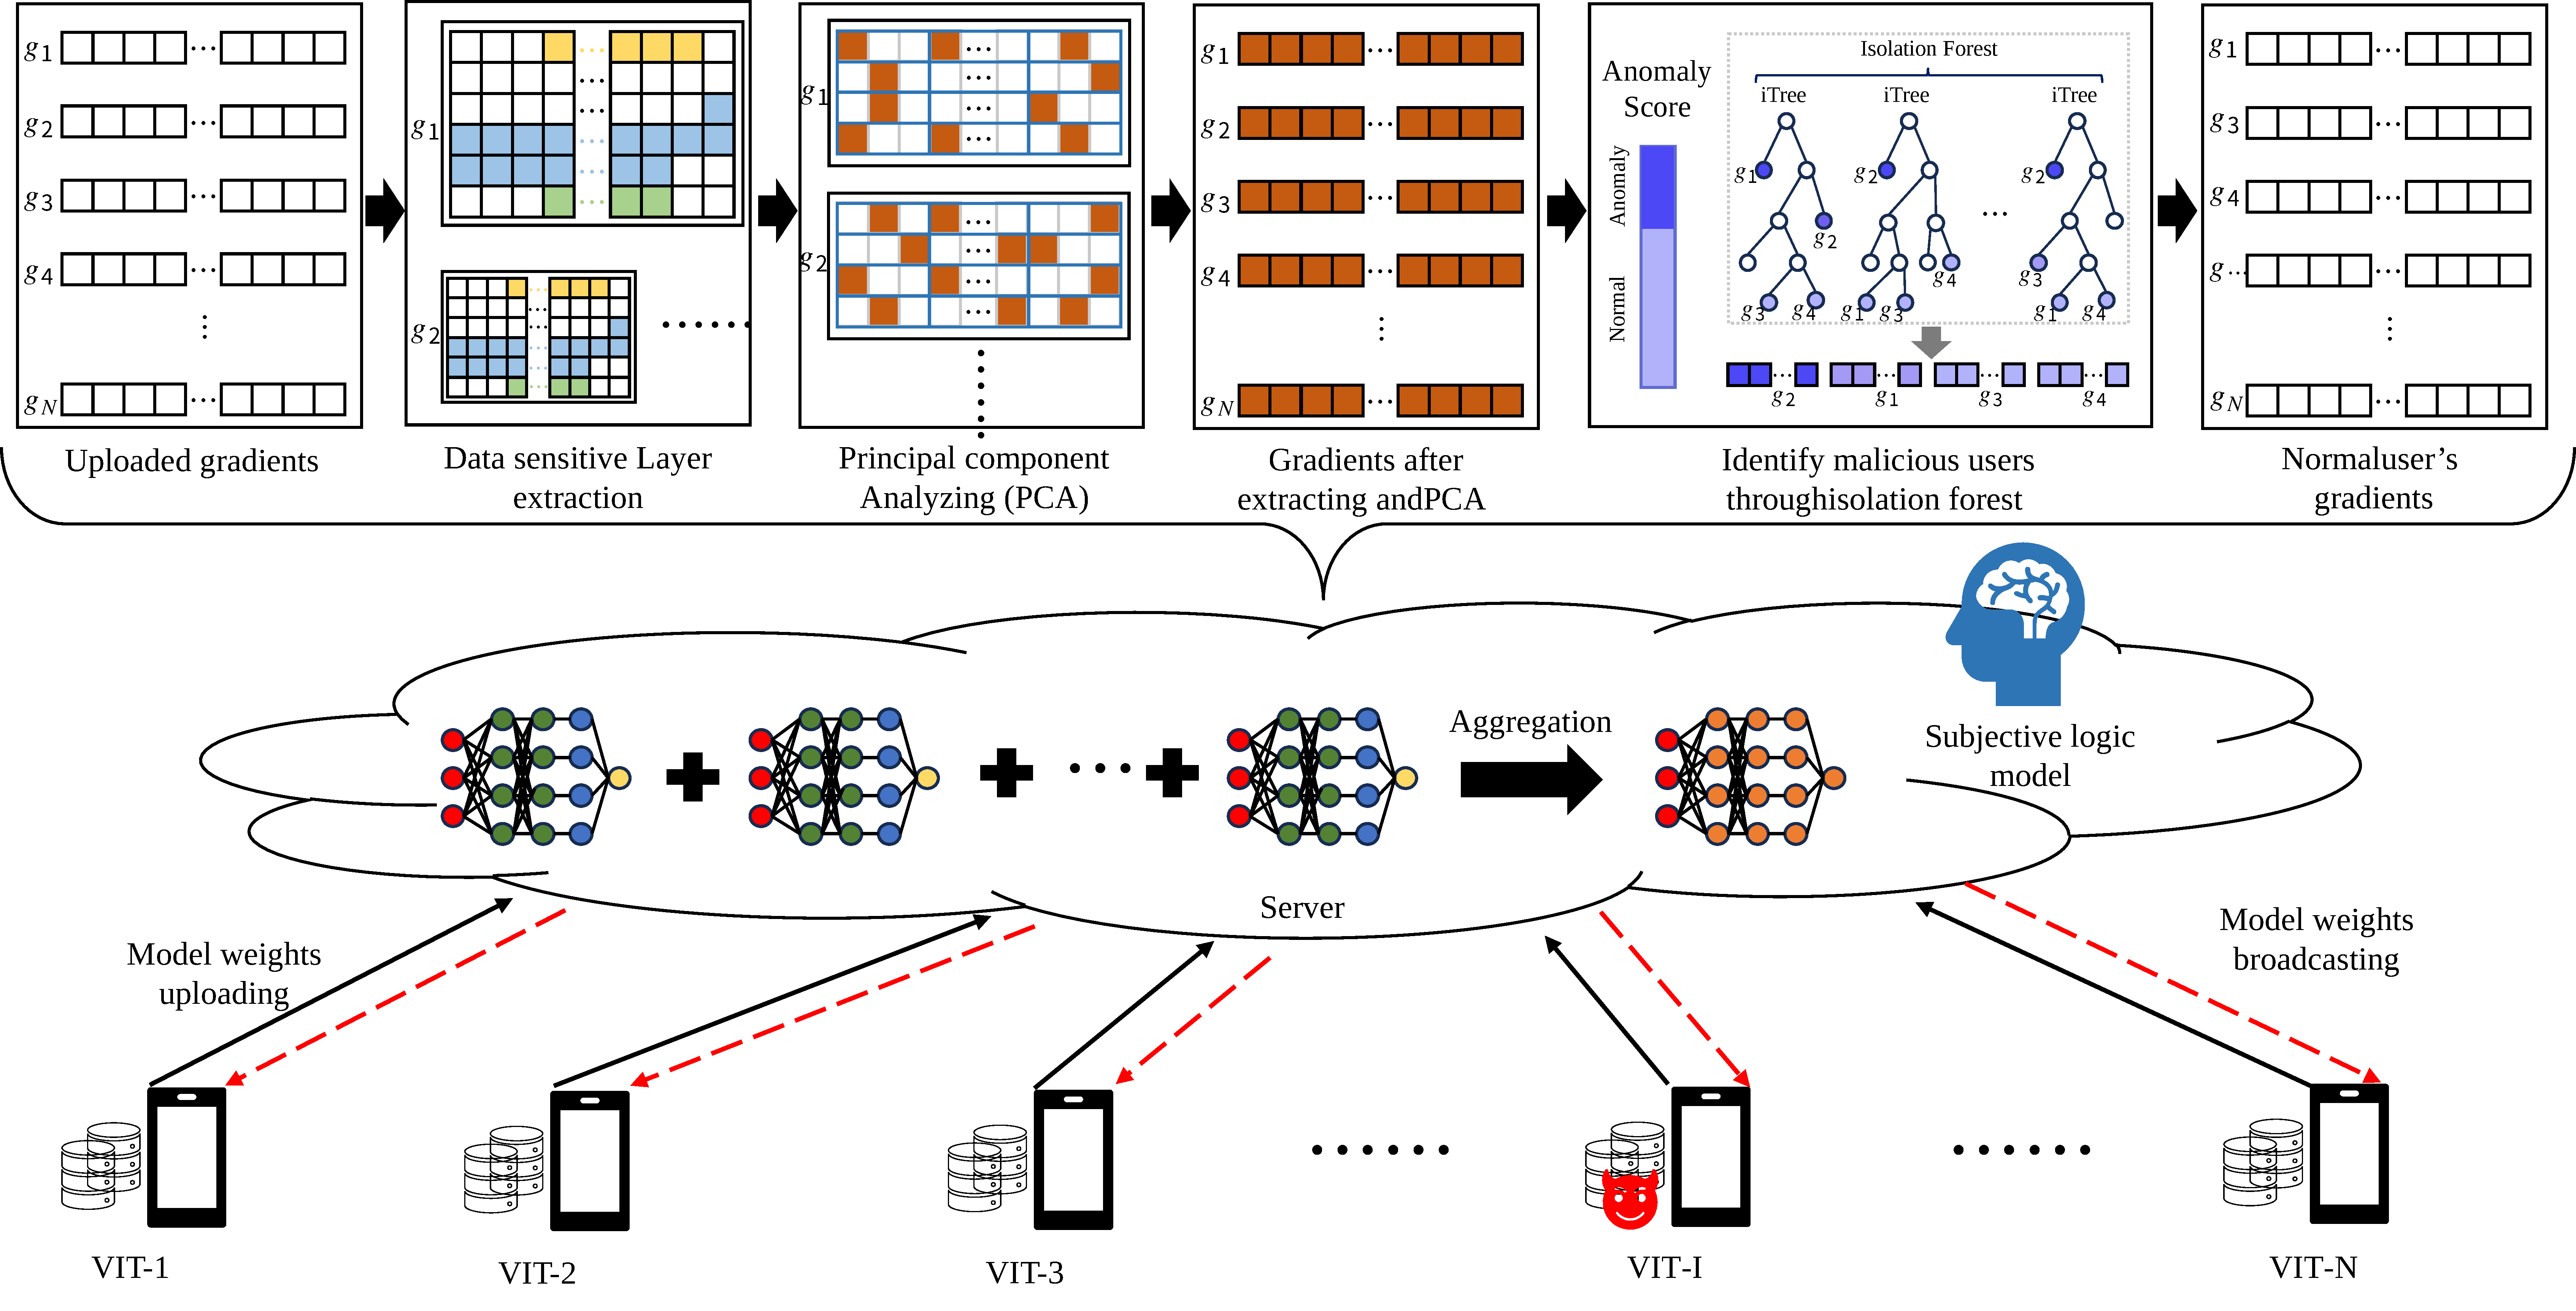
\includegraphics[width=\figTotalScene]{pics/000-totalScene.pdf}}
    \caption{ViT Total Scene}
    \label{fig:totalScene}
\end{figure*}

% 图\hyperref[fig:totalScene]{\ref{fig:totalScene}}展示了ViT-MGI算法的整个流程。首先,ViT-MGI收集各个客户端上传上来的梯度变化结果,然后根据\hyperref[exp:exp_layer]{§\ref{exp:exp_layer}}得出的结论将攻击识别所关注的层提取出来。如图\hyperref[fig:totalScene]{\ref{fig:totalScene}}所示,对于某个客户端$c_i$,我们将其上传到中央服务器的梯度记为$g_i$,ViT-MGI首先将$g_i$中的encoder层5的attention.attention.key.bias等全部提取出来重新拼接到一个向量中并记为$\phi(g_i)$,之后使用主成分分析算法对这些数据中的主成分进行分析。

% Figure \hyperref[fig:totalScene]{\ref{fig:totalScene}} illustrates the entire process of the ViT-MGI algorithm. First, ViT-MGI collects the gradient updates uploaded by various clients and then extracts the layers of interest for attack detection based on the conclusions derived in \hyperref[exp:exp_layer]{§\ref{exp:exp_layer}}. As shown in Figure \hyperref[fig:totalScene]{\ref{fig:totalScene}}, for a given client $c_i$, we denote the gradient uploaded to the central server as $g_i$. ViT-MGI initially extracts all elements such as the attention.attention.key.bias from encoder layer 5 within $g_i$, reassembling them into a vector denoted as $\phi(g_i)$. Next, it applies the principal component analysis (PCA) algorithm to analyze the principal components within this data.

% % 对于提取特征层之后的权重$\phi(g_i)$,我们使用主成分分析算法对其进行二次降维,将降维之后的权重记为$\phi'(g_i)$。主成分分析通过线性变换将高维数据投影到低维空间,保留数据中最重要的变化信息。通过这种方式,ViT-MGI算法能够在保留数据主要信息的同时,显著减少数据的维度,从而提高后续攻击检测算法的效率和准确性。

% % 接下来,使用隔离森林算法对降维后的数据进行分析。隔离森林算法通过随机选择特征和分割值来构建树结构,以便有效地隔离数据点。对每个客户端的降维数据 $\phi'(g_i)$ 进行隔离森林分析,得到异常评分 $s_i$,用于识别潜在的恶意客户端。具体来说,隔离森林算法会计算每个数据点被隔离的平均路径长度,异常数据点的路径长度通常较短。

% % 最后,采用主观逻辑模型对每个客户端进行评分。主观逻辑模型根据客户端的历史行为和当前表现,计算其可信度评分 $\sigma_i$。评分结果用于筛选可信客户端,并将这些客户端的梯度加权合并到全局模型中。

% For the extracted feature weights $\phi(g_i)$, we apply the PCA algorithm for a second round of dimensionality reduction, resulting in the reduced weights denoted as $\phi'(g_i)$. PCA performs a linear transformation to project high-dimensional data into a lower-dimensional space, preserving the most significant variations in the data. This approach allows the ViT-MGI algorithm to retain the essential information while significantly reducing the data's dimensionality, thereby improving the efficiency and accuracy of subsequent attack detection algorithms.

% Next, the reduced data is analyzed using the isolation forest algorithm. The isolation forest algorithm constructs a tree structure by randomly selecting features and split values to effectively isolate data points. Each client’s reduced data $\phi'(g_i)$ is analyzed using the isolation forest to obtain an anomaly score $s_i$, which is used to identify potential malicious clients. Specifically, the isolation forest algorithm calculates the average path length required to isolate each data point, with anomalous data points typically having shorter path lengths.

% Finally, a subjective logic model is employed to score each client. The subjective logic model evaluates the trustworthiness score $\sigma_i$ of each client based on their historical behavior and current performance. These scores are used to filter trustworthy clients, and the gradients of these clients are weighted and aggregated into the global model.

Figure \hyperref[fig:totalScene]{\ref{fig:totalScene}} illustrates the entire process of the ViT-MGI algorithm. ViT-MGI first collects gradient updates from various clients and extracts the layers of interest for attack detection based on the conclusions in \hyperref[fig:totalScene]{\ref{fig:totalScene}}. For a given client $c_i$, the gradient uploaded to the central server is denoted as $g_i$. ViT-MGI extracts elements like attention.attention.key.bias from encoder layer 5 within $g_i$, reassembling them into a vector denoted as $\phi(g_i)$. It then applies principal component analysis (PCA) to analyze the principal components within this data.

For the extracted feature weights $\phi(g_i)$, PCA is applied for dimensionality reduction, resulting in reduced weights denoted as $\phi'(g_i)$. Then, the reduced data is analyzed using the isolation forest algorithm. Each client’s reduced data $\phi'(g_i)$ is analyzed to obtain an anomaly score $s_i$, identifying potential malicious clients. The isolation forest calculates the average path length to isolate each data point.

Finally, a subjective logic model evaluates the trustworthiness score $\sigma_i$ of each client based on historical behavior and current performance. These scores filter trustworthy clients, whose gradients are then weighted and aggregated into the global model.

% \subsection{特征层提取}
\subsection{Feature Layer Extraction}
\label{sec:method_layer}

% 就模型ViT-B/16而言,对于某个客户端$c_i$,其上传到中央服务器的梯度变化数量为$85806346$个。将其上传到中央服务器的梯度记为$g_i$,ViT-MGI首先将通过实验\hyperref[exp:exp_layer]{§\ref{exp:exp_layer}}得到的对于攻击敏感的层全部提取出来,之后将其重新拼接到一个向量中。我们将这些提取出来的更加有效的数据记为$\phi(g_i)$,则经过特征层提取这一步的操作后,每个客户端的参数数量将由$g_i$的$85806346$个减少到$\phi(g_i)$的$\frac1{10}$左右,具体的提取方法如\hyperref[alg:layerExtra]{Algorithm \ref{alg:layerExtra}}所示。

% 这些特征层是由我们经过一系列实验得到的。在实验\hyperref[exp:exp_layer]{§\ref{exp:exp_layer}}中,我们将ViT模型划分为了$200$个层,其中每个层大约平均就只有几十万个参数。

For the ViT-B/16 model, the number of gradient changes uploaded to the central server by a client $c_i$ is 85,806,346. Denoting the gradients uploaded to the central server as $g_i$, ViT-MGI first extracts all layers sensitive to attacks based on experiments described in \hyperref[exp:exp_layer]{§\ref{exp:exp_layer}}, and then reassembles these extracted layers into a single vector. We denote these more effective extracted data as $\phi(g_i)$. After the feature layer extraction step, the number of parameters for each client is reduced from 85,806,346 in $g_i$ to approximately $\frac1{10}$ in $\phi(g_i)$. The specific extraction method is shown in \hyperref[alg:layerExtra]{Algorithm \ref{alg:layerExtra}}.

These feature layers are identified through a series of experiments. In experiment \hyperref[exp:exp_layer]{§\ref{exp:exp_layer}}, we divided the ViT model into 200 layers, with each layer averaging only a few hundred thousand parameters.

% \begin{algorithm}
%     \caption{特征层提取}
%     \label{alg:example}
%     \begin{algorithmic}[1]
%         \Require $g_i$ - 第$i$个客户端上传的梯度; $L_{keep}$ - 要保留的层
%         \Ensure $\phi(g_i)$ - 提取特征层后的梯度
%         \Function{Extract}{$g_i, L_{keep}$}
%         \For{$l\in g_i.layers()$}
%             \If{$l.name\in L_{keep}$}
%                 \State $\phi_i\gets l$
%             \EndIf
%         \EndFor
%         \State $\phi(g_i)\gets Concatenate(\{\phi_i | i=1, 2, \cdots, len(L_{keep}) \})$
%         \Return $\phi(g_i)$
%         \EndFunction
%     \end{algorithmic}
% \end{algorithm}

% \begin{algorithm}
%     \caption{特征层提取}
%     \label{alg:layerExtra}
%     \begin{algorithmic}[1]
%         \Require $g_i$ - 第$i$个客户端上传的梯度; $L_{keep}$ - 要保留的层
%         \Ensure $\phi(g_i)$ - 提取特征层后的梯度
%         \Function{Extract}{$g_i, L_{keep}$}
%             \State $\phi(g_i)\gets\emptyset$
%             \For{$l\in g_i.layers()$}
%                 \If{$l.name \in L_{keep}$}
%                     \State $\phi(g_i).append(l)$
%                 \EndIf
%             \EndFor
%             \State \Return $\phi(g_i)$
%         \EndFunction
%     \end{algorithmic}
% \end{algorithm}

\begin{algorithm}
    \caption{Feature Layer Extraction}
    \label{alg:layerExtra}
    \begin{algorithmic}[1]
        \Require $g_i$ - Gradient uploaded by client $i$; $L_{keep}$ - Layers to keep
        \Ensure $\phi(g_i)$ - Gradient after feature layer extraction
        \Function{Extract}{$g_i, L_{keep}$}
            \State $\phi(g_i) \gets \emptyset$
            \For{$l \in g_i.layers()$}
                \If{$l.name \in L_{keep}$}
                    \State $\phi(g_i).append(l)$
                \EndIf
            \EndFor
            \State \Return $\phi(g_i)$
        \EndFunction
    \end{algorithmic}
\end{algorithm}


% \subsection{主成分分析}
\subsection{Principal Component Analysis}
\label{sec:method_PCA}

% % 在完成特征层提取后,我们得到了每个客户端上传的特征向量$\phi(g_i)$。为了进一步简化数据结构并保留主要信息,ViT-MGI算法使用主成分分析对这些特征向量进行处理。

% After completing the feature layer extraction, we obtain the feature vectors $\phi(g_i)$ uploaded by each client. To further simplify the data structure and retain the primary information, the ViT-MGI algorithm employs Principal Component Analysis (PCA) to process these feature vectors.

% % PCA是一种常用的降维技术,通过将高维数据投影到一个低维空间中,保留数据中最重要的变化信息。具体来说,PCA通过线性变换将数据转化为一组新的不相关变量,这些变量称为主成分。主成分按其解释的方差大小排序,前几个主成分保留了数据中的主要信息,从而减少了数据维度。

% % 对于每个客户端的特征向量$\phi(g_i)$,我们首先对其进行中心化处理,即减去其均值:

% % \[
% % \phi(g_i) = \phi(g_i) - \bar{\phi}
% % \]

% % 其中,$\bar{\phi}$是所有客户端上传的特征向量的均值。接下来,计算协方差矩阵:

% % \[
% % \mathbf{C} = \frac{1}{N} \sum_{i=1}^N \phi(g_i) \phi(g_i)^T
% % \]

% % 然后,对协方差矩阵$\mathbf{C}$进行特征值分解,得到特征值和特征向量:

% % \[
% % \mathbf{C} = \mathbf{V} \mathbf{\Lambda} \mathbf{V}^T
% % \]

% % 其中,$\mathbf{\Lambda}$是对角矩阵,其对角元素是协方差矩阵的特征值,$\mathbf{V}$是特征向量矩阵。特征向量矩阵$\mathbf{V}$的每一列是一个主成分的方向。我们选择前$r$个最大的特征值对应的特征向量构成的子空间:

% % \[
% % \mathbf{V}_r = [\mathbf{v}_1, \mathbf{v}_2, \ldots, \mathbf{v}_r]
% % \]

% % 将原始数据投影到该子空间中,得到降维后的数据:

% % \[
% % \phi'(g_i) = \mathbf{V}_r^T \phi(g_i)
% % \]

% % PCA是一种常用的降维技术,通过线性变换将高维数据投影到低维空间中,保留数据中最重要的变化信息。对于每个客户端的特征向量,我们首先进行中心化处理,然后计算协方差矩阵,并进行特征值分解,选择前几个最大的特征值对应的特征向量构成的子空间,将原始数据投影到该子空间中,得到降维后的数据,从而提高后续攻击检测算法的效率和准确性。

% PCA is a commonly used dimensionality reduction technique that projects high-dimensional data into a low-dimensional space through linear transformation, retaining the most significant variation information in the data. For each client's feature vector, we first perform centralization, then calculate the covariance matrix, and perform eigenvalue decomposition. We select the subspace formed by the eigenvectors corresponding to the largest eigenvalues and project the original data into this subspace to obtain the reduced-dimension data, thereby improving the efficiency and accuracy of subsequent attack detection algorithms.

% % 通过这种方式,ViT-MGI算法能够在保留数据主要信息的同时,显著减少数据的维度,从而提高后续攻击检测算法的效率和准确性。

% In this way, the ViT-MGI algorithm can significantly reduce the dimensionality of the data while retaining the main information, thereby improving the efficiency and accuracy of subsequent attack detection algorithms.

% After feature layer extraction, we obtain the feature vectors $\phi(g_i)$ from each client. The ViT-MGI algorithm then uses Principal Component Analysis (PCA) to simplify the data structure while retaining primary information.

% PCA is a dimensionality reduction technique that projects high-dimensional data into a low-dimensional space, capturing the most significant variations. For each client's feature vector, we centralize the data, compute the covariance matrix, and perform eigenvalue decomposition. We select the subspace formed by the eigenvectors with the largest eigenvalues, projecting the original data into this subspace to obtain reduced-dimension data.

% This process significantly reduces data dimensionality while retaining essential information, thus enhancing the efficiency and accuracy of subsequent attack detection algorithms.

% After feature layer extraction, we obtain the feature vectors $\phi(g_i)$ from each client. The ViT-MGI algorithm then employs Principal Component Analysis (PCA) to simplify the data structure while retaining primary information.

% PCA reduces dimensionality by projecting high-dimensional data into a lower-dimensional space, capturing significant variations. For each client's feature vector, we centralize the data, compute the covariance matrix, and perform eigenvalue decomposition. We then project the original data into the subspace formed by the eigenvectors with the largest eigenvalues, obtaining reduced-dimension data.

% This process retains essential information while significantly reducing data dimensionality, enhancing the efficiency and accuracy of subsequent attack detection algorithms.

After feature layer extraction, the ViT-MGI algorithm uses PCA to simplify the data structure while retaining primary information. PCA reduces dimensionality by projecting high-dimensional data into a lower-dimensional space, capturing significant variations. This process retains essential information and enhances the efficiency and accuracy of subsequent attack detection algorithms.

% \subsection{隔离森林}
\subsection{Isolation Forest}
\label{sec:method_forest}

% 在完成主成分分析(PCA)后,我们得到了降维后的数据$\phi'(g_i)$。为了识别潜在的恶意客户端,ViT-MGI算法使用隔离森林(Isolation Forest)算法对这些降维后的数据进行异常检测。

% After completing the PCA, we obtain the dimensionally reduced data $\phi'(g_i)$. To identify potential malicious clients, the ViT-MGI algorithm uses the Isolation Forest algorithm to perform anomaly detection on these reduced data.

% % 隔离森林是一种基于树结构的无监督异常检测算法,其核心思想是通过随机选择特征和分割值构建树结构,以便有效地隔离数据点。异常数据点通常更容易被隔离,因为它们在树结构中的路径长度较短。具体来说,隔离森林算法的步骤如下:

% % 1. 构建森林:首先,随机选择一个子样本集,并从中构建多棵隔离树(iTree)。每棵树通过随机选择特征和分割点来分割数据,直到所有数据点都被完全隔离,或者达到预定的最大树深度。

% % 2. 计算路径长度:对于每个数据点,计算其在每棵树中的路径长度,即从根节点到叶节点的距离。异常数据点的平均路径长度较短,因为它们更容易被隔离。

% % 3. 计算异常评分:根据路径长度计算每个数据点的异常评分。具体来说,假设数据点$x$在隔离树中的平均路径长度为$h(x)$,则其异常评分$s(x)$定义为:
% %    \[
% %    s(x) = 2^{-\frac{h(x)}{c(n)}}
% %    \]
% % 其中,$c(n)$是一个调整因子,$n$为数据集的样本数量。异常评分$s(x)$越接近1,表示数据点越可能是异常点。

% % 隔离森林是一种基于树结构的无监督异常检测算法,通过随机选择特征和分割值构建多棵树,计算每个数据点在树中的路径长度,并根据路径长度计算异常评分,评分越高表示数据点越可能是异常点。

% Isolation Forest is an unsupervised anomaly detection algorithm based on tree structures. It constructs multiple trees by randomly selecting features and split values, calculates the path length of each data point within the trees, and computes an anomaly score based on the path length. Higher scores indicate a higher likelihood of the data point being an anomaly.

% % 在ViT-MGI算法中,我们对每个客户端的降维数据$\phi'(g_i)$进行隔离森林分析,得到每个客户端的异常评分$s_i$。这些异常评分用于识别潜在的恶意客户端。在后续步骤中,我们将结合这些评分和主观逻辑模型计算每个客户端的可信度评分$\sigma_i$,从而筛选出可信的客户端进行全局模型更新。

% In the ViT-MGI algorithm, we perform Isolation Forest analysis on the dimensionally reduced data $\phi'(g_i)$ for each client, obtaining an anomaly score $s_i$ for each client. These anomaly scores are used to identify potential malicious clients. In subsequent steps, we combine these scores with a subjective logic model to calculate a credibility score $\sigma_i$ for each client, thereby selecting trustworthy clients for global model updates.

% After PCA, we obtain the dimensionally reduced data $\phi'(g_i)$. The ViT-MGI algorithm then uses the Isolation Forest algorithm to detect anomalies and identify potential malicious clients.

% Isolation Forest is an unsupervised anomaly detection algorithm that constructs trees by randomly selecting features and split values. It calculates the path length of each data point within the trees and computes an anomaly score based on the path length, with higher scores indicating a higher likelihood of being an anomaly.

% In the ViT-MGI algorithm, we analyze the reduced data $\phi'(g_i)$ for each client using Isolation Forest, obtaining an anomaly score $s_i$. These scores help identify potential malicious clients. We then combine these scores with a subjective logic model to calculate a credibility score $\sigma_i$, selecting trustworthy clients for global model updates.

After PCA, the ViT-MGI algorithm uses the Isolation Forest algorithm to detect anomalies and identify potential malicious clients. Isolation Forest constructs trees by randomly selecting features and split values, calculating anomaly scores based on the path lengths within the trees. These scores help identify potential malicious clients, which are then further analyzed using a subjective logic model to select trustworthy clients for global model updates.

% \subsection{主观逻辑模型}
\subsection{Subjective Logic Model}
\label{sec:method_subjective}

% 在使用隔离森林算法对降维后的数据进行异常检测并获得每个客户端的异常评分$s_i$之后,ViT-MGI算法进一步采用主观逻辑模型(Subjective Logic Model, SLM)来计算每个客户端的可信度评分$\sigma_i$。

After performing anomaly detection on the dimensionally reduced data using the Isolation Forest algorithm and obtaining an anomaly score $s_i$ for each client, the ViT-MGI algorithm further employs the Subjective Logic Model (SLM) to calculate a credibility score $\sigma_i$ for each client.

% 主观逻辑模型是一种用于处理不确定性和主观意见的数学框架,通过结合历史行为和当前表现来计算每个客户端的可信度评分。具体来说,主观逻辑模型使用信任度(belief)、不信任度(disbelief)和不确定度(uncertainty)三个参数来表示可信度评分。对于每个客户端$c_i$,这些参数可以根据其历史行为和异常评分来计算。

% 1. 信任度(Belief):信任度表示对客户端行为的信任程度。可以根据客户端在过去多次训练中的良好表现来估计。例如,客户端上传的模型更新在过去多次迭代中表现稳定且有效,则其信任度较高。

% 2. 不信任度(Disbelief):不信任度表示对客户端行为的不信任程度。可以根据隔离森林算法检测到的异常评分$s_i$来估计。如果客户端的异常评分较高,则其不信任度也较高。

% 3. 不确定度(Uncertainty):不确定度表示对客户端行为的不确定性。当缺乏足够的历史数据或当前表现不明显时,不确定度较高。

% 主观逻辑模型结合这三个参数,计算每个客户端的综合可信度评分$\sigma_i$。具体计算公式如下:
% \[
% \sigma_i = \frac{b_i}{b_i + d_i + u_i}
% \]
% 其中,$b_i$、$d_i$和$u_i$分别表示客户端$c_i$的信任度、不信任度和不确定度。

% 根据计算得到的可信度评分$\sigma_i$,我们可以筛选出可信的客户端进行全局模型更新。具体地,全局模型更新规则为:
% \[
% \theta \leftarrow \theta - \eta \sum_{i=1}^N w_i \Delta \theta_i
% \]
% 其中,$w_i$为第$i$个客户端的权重,根据其可信度评分$\sigma_i$确定。

% 主观逻辑模型通过结合信任度、不信任度和不确定度三个参数,根据客户端的历史行为和当前表现计算其可信度评分,从而筛选出可信的客户端进行全局模型更新。

The Subjective Logic Model\cite{Subjective_Logic_Model} calculates the trustworthiness score of each client by combining three parameters: belief, disbelief, and uncertainty, based on the client's historical behavior and current performance. This score is then used to select trustworthy clients for updating the global model.

% 通过主观逻辑模型,ViT-MGI算法能够更有效地识别并筛选出可信的客户端,确保全局模型的鲁棒性和准确性。

Through the Subjective Logic Model, the ViT-MGI algorithm can more effectively identify and filter out trustworthy clients, ensuring the robustness and accuracy of the global model.

% \begin{algorithm}
%     \caption{ViT-MGI 总流程}
%     \label{alg:vit_mgi}
%     \begin{algorithmic}[1]
%         \Require $G = \{g_i\}$ - 各客户端上传的梯度集合; $L_{keep}$ - 要保留的特征层
%         \Ensure $\theta$ - 更新后的全局模型参数
%         \Function{ViT-MGI}{$g_i, L_{keep}$}
%             \State 初始化全局模型参数 $\theta$
%             \For{每个通信轮次 $t$}
%                 \State \textcolor{blue}{\# 特征层提取}
%                 \For{每个客户端 $c_i \in G$}
%                     \State 提取 $g_i$ 中的特征层,得到 $\phi(g_i)$
%                 \EndFor
                
%                 \State \textcolor{blue}{\# PCA}
%                 \For{每个客户端 $c_i \in G$}
%                     \State 对 $\phi(g_i)$ 进行中心化处理
%                     \State 计算协方差矩阵并进行特征值分解
%                     \State 得到降维后的数据 $\phi'(g_i)$
%                 \EndFor
                
%                 \State \textcolor{blue}{\# 隔离森林 (Isolation Forest)}
%                 \For{每个客户端 $c_i \in G$}
%                     \State 使用隔离森林算法对 $\phi'(g_i)$ 进行异常检测,得到异常评分 $s_i$
%                 \EndFor
                
%                 \State \textcolor{blue}{\# 主观逻辑模型 (SLM)}
%                 \For{每个客户端 $c_i \in G$}
%                     \State 根据历史行为和异常评分 $s_i$ 计算可信度评分 $\sigma_i$
%                     \State 根据 $\sigma_i$ 计算权重 $w_i$
%                 \EndFor
                
%                 \State \textcolor{blue}{\# 全局模型更新}
%                 \State 计算加权合并后的全局模型更新 $\Delta \theta = \sum_{i=1}^N w_i \Delta \theta_i$
%                 \State 更新全局模型参数 $\theta \leftarrow \theta - \eta \Delta \theta$
%             \EndFor
%         \EndFunction
%         \State \Return $\theta$
%     \end{algorithmic}
% \end{algorithm}



% (也是总分,技术上是怎么实现的)

% \textcolor{red}{TODO:} 总的方案图

% \textcolor{red}{TODO:} 能体现细节的图

% (至少一张图,可2张3张,一张大的(总的方案图),可加小(细节)图)

% (最后也可给个伪代码 )

% \textcolor{red}{明后天写完}

\section{Experiments}
\label{sec:exp}

% 池化+PCA的实验 对比 PCA的实验,发现只有耗时减少了,但准确率会下降。证明池化技术不适用于具有大量参数的ViT的拜占庭攻击检测。

% \begin{itemize}
%     \item \textbf{实际标签(True Labels)}: 每个客户端的实际恶意程度(0 表示良性,1 表示恶意)。
%     \item \textbf{预测概率(Predicted Probabilities)}: 每个客户端的恶意概率预测值(介于 0 到 1 之间)。
% \end{itemize}

% Log Loss(对数损失)衡量的是模型预测的概率与实际标签之间的不一致性,数值越小越好。

% \begin{equation}
% \text{Log Loss} = -\frac{1}{N} \sum_{i=1}^{N} [y_i \log(p_i) + (1 - y_i) \log(1 - p_i)]
% \end{equation}

% 其中,$y_i$ 为实际标签(0 或 1),$p_i$ 为预测的恶意概率。

% Brier Score(布雷尔分数)衡量的是预测概率与实际标签之间的均方误差,数值越小越好。

% \begin{equation}
% \text{Brier Score} = \frac{1}{N} \sum_{i=1}^{N} (p_i - y_i)^2
% \end{equation}

% AUC-ROC受试者工作特征曲线下面积衡量的是分类器在不同阈值下的性能,数值越接近1,分类器性能越好。

% \begin{equation}
% \text{AUC} = \int_0^1 \text{TPR}(\text{FPR}) \, d(\text{FPR})
% \end{equation}

% 其中,TPR 为真阳性率,FPR 为假阳性率。

% PRC-AUC(精确率-召回率曲线下面积)衡量的是分类器在不同阈值下的精确率和召回率之间的权衡。

% \begin{equation}
% \text{PRC-AUC} = \int_0^1 \text{Precision}(\text{Recall}) \, d(\text{Recall})
% \end{equation}

% Calibration Plot(校准曲线)展示的是预测概率和实际概率的一致性。校准曲线越接近45度线,预测概率越准确。

% \begin{enumerate}
%     \item \textbf{数据准备}:
%     \begin{itemize}
%         \item 收集并标注每个客户端的实际恶意程度(0 或 1)。
%         \item 使用各算法对每个客户端进行恶意概率预测。
%     \end{itemize}

%     \item \textbf{评估指标计算}:
%     \begin{itemize}
%         \item 计算每个算法在各个指标(Log Loss、Brier Score、AUC-ROC、PRC-AUC)上的表现。
%     \end{itemize}

%     \item \textbf{校准曲线绘制}:
%     \begin{itemize}
%         \item 绘制预测概率与实际概率的校准曲线,评估预测概率的准确性。
%     \end{itemize}

%     \item \textbf{结果分析}:
%     \begin{itemize}
%         \item 对比各算法在不同评估指标上的性能。
%         \item 使用可视化方法展示不同算法的优劣(如绘制ROC曲线、PR曲线、校准曲线)。
%     \end{itemize}
% \end{enumerate}

% \subsection{实验设置}
\subsection{Experimental Setup}
\label{exp:settings}

% 本实验在一台配置高性能硬件的Ubuntu 20.04.3 LTS操作系统的计算机上进行,具体配置如下:

% 操作系统:Ubuntu 20.04.3 LTS,内核版本 5.15.0-73-generic
% CPU:Intel(R) Core(TM) i9-10940X CPU @ 3.30GHz,28核,最大频率 4.8GHz
% 内存:128GB DDR4,2933 MT/s
% GPU:2 x NVIDIA GeForce RTX 3090,显存各 24GB,驱动版本 470.239.06,CUDA 版本 11.4
% 存储:SSD,提供高速数据读写支持
% 为了确保实验结果的可靠性和再现性,我们使用了标准的数据集,包括MNIST数据集和一个大型工业产品推荐数据集。实验中使用的具体硬件配置能够提供充足的计算资源,支持大规模深度学习模型的训练和复杂算法的测试。

% 我们的实验在一台操作系统为Ubuntu 20.04.3 LTS的计算机上进行,CPU为Intel i9-10940X 28核;内存为128GB DDR4;显卡为2张NVIDIA GeForce RTX 3090,显存各 24GB。我们实验使用的模型为ViT-B/16,并在ViT-L/16、ViT-H/14上进行了验证。我们实验使用的数据集为CIFAR-10,同时在MNIST、OrganAMNIST上进行了验证。对于攻击的方式,我们验证了包括属于拜占庭攻击的梯度上升攻击、标签翻转攻击以及属于非拜占庭攻击的后门植入攻击等多种攻击方式。关于防御方式,我们使用并对比了ViT-MGI、PCA、隔离森林、池化放大\cite{betterTogether}+PCA、池化放大+隔离森林,以及常用的或最新的余弦相似度计算等算法。最终证实了我们算法的有效性。在我们的开源仓库中保留了ViT-MGI研究过程中的每次的实验记录与结果。

Our experiments were conducted on a computer running Ubuntu 20.04.3 LTS, equipped with an Intel i9-10940X 28-core CPU, 128GB DDR4 memory, and two NVIDIA GeForce RTX 3090 GPUs, each with 24GB of VRAM. We used the ViT-B/16 model for our experiments and validated our findings on ViT-L/16 and ViT-H/14 models. The datasets used in our experiments included CIFAR-10, with additional validation on MNIST and OrganAMNIST. We evaluated various attack methods, including Byzantine attacks like gradient ascent attacks and label flipping attacks, as well as non-Byzantine attacks such as backdoor injections. For defense methods, we used and compared ViT-MGI, PCA, Isolation Forest, Pooling Amplification\cite{betterTogether}+PCA, Pooling Amplification+Isolation Forest, and commonly used or state-of-the-art cosine similarity calculations. The effectiveness of our algorithm was confirmed through these comparisons. Detailed experimental records and results from our ViT-MGI research are preserved in our open-source repository.

% \subsection{攻击有效性实验}
\subsection{Attack Effectiveness Experiment}
\label{exp:attack}

% 为了能够更好地进一步实验,我们决定首先搭建好联邦学习训练ViT的框架。我们使用PyTorch作为深度学习库,使用ViT-L/16的预训练模型和CIFAR-10数据集,使用串行的方式依次模拟各个客户端,每个客户端都有自己独自的数据集,它们在本地训练结束后将梯度变化上传到中央服务器中。经过一系列的调参后,模型能够在较短的时间内,从最初的大约10\%的准确率逐渐上升到大约97\%的准确率。

To conduct further experiments, we first established a framework for federated learning with ViT. We used PyTorch as our deep learning library, employed the pre-trained ViT-L/16 model, and utilized the CIFAR-10 dataset. We simulated each client sequentially, with each client having its own dataset. After local training, clients uploaded their gradient updates to the central server. After a series of parameter adjustments, the model's accuracy gradually increased from approximately 10\% to about 97\% in a relatively short time.

\subsubsection{\textbf{Gradient Ascent Attack}}
\label{exp:attack:grad}

% 我们在正常的联邦学习框架基础上分别进行了不加任何防御的梯度上升攻击、标签翻转攻击以及后门植入攻击,结果发现对于梯度上升攻击,若不进行防御,则在20\%的攻击者与较小的攻击力度的情况下,模型准确率上升明显减慢。如图\hyperref[fig:gradAscent]{\ref{fig:gradAscent}}所示,攻击者的比例都是20\%。当攻击者把本地训练得到的梯度变化进行取反操作时,发现模型准确率的上升有一定程度的减缓;当攻击者把本地的梯度变化乘以$-2$后上传时,发现模型准确率的上升速率进一步下降;而当攻击者把本地梯度变化乘以$-3$再上传时,可以发现模型已经无法正常工作。图\hyperref[fig:gradAscent]{\ref{fig:gradAscent}}中蓝色曲线显示的是没有攻击者时的训练结果,橘色曲线显示的是梯度取反的攻击结果,绿色、红色和紫色的曲线显示的分别是梯度乘以$-2$、$-3$、$-4$时的训练结果。

% 我们在正常的联邦学习框架基础上进行了梯度上升攻击实验。若不进行防御,当20\%的攻击者将本地训练得到的梯度变化取反或乘以负数上传时,模型准确率显著下降。图\hyperref[fig:gradAscent]{\ref{fig:gradAscent}}中蓝色曲线显示的是没有攻击者时的训练准确率结果,橘色、绿色、红色和紫色的曲线显示的分别是梯度乘以$-1$、$-2$、$-3$、$-4$时的训练结果。可以看出攻击力度越大准确率下降越明显,这说明梯度上升攻击是有效的。

\begin{figure}[htbp]
    \centerline{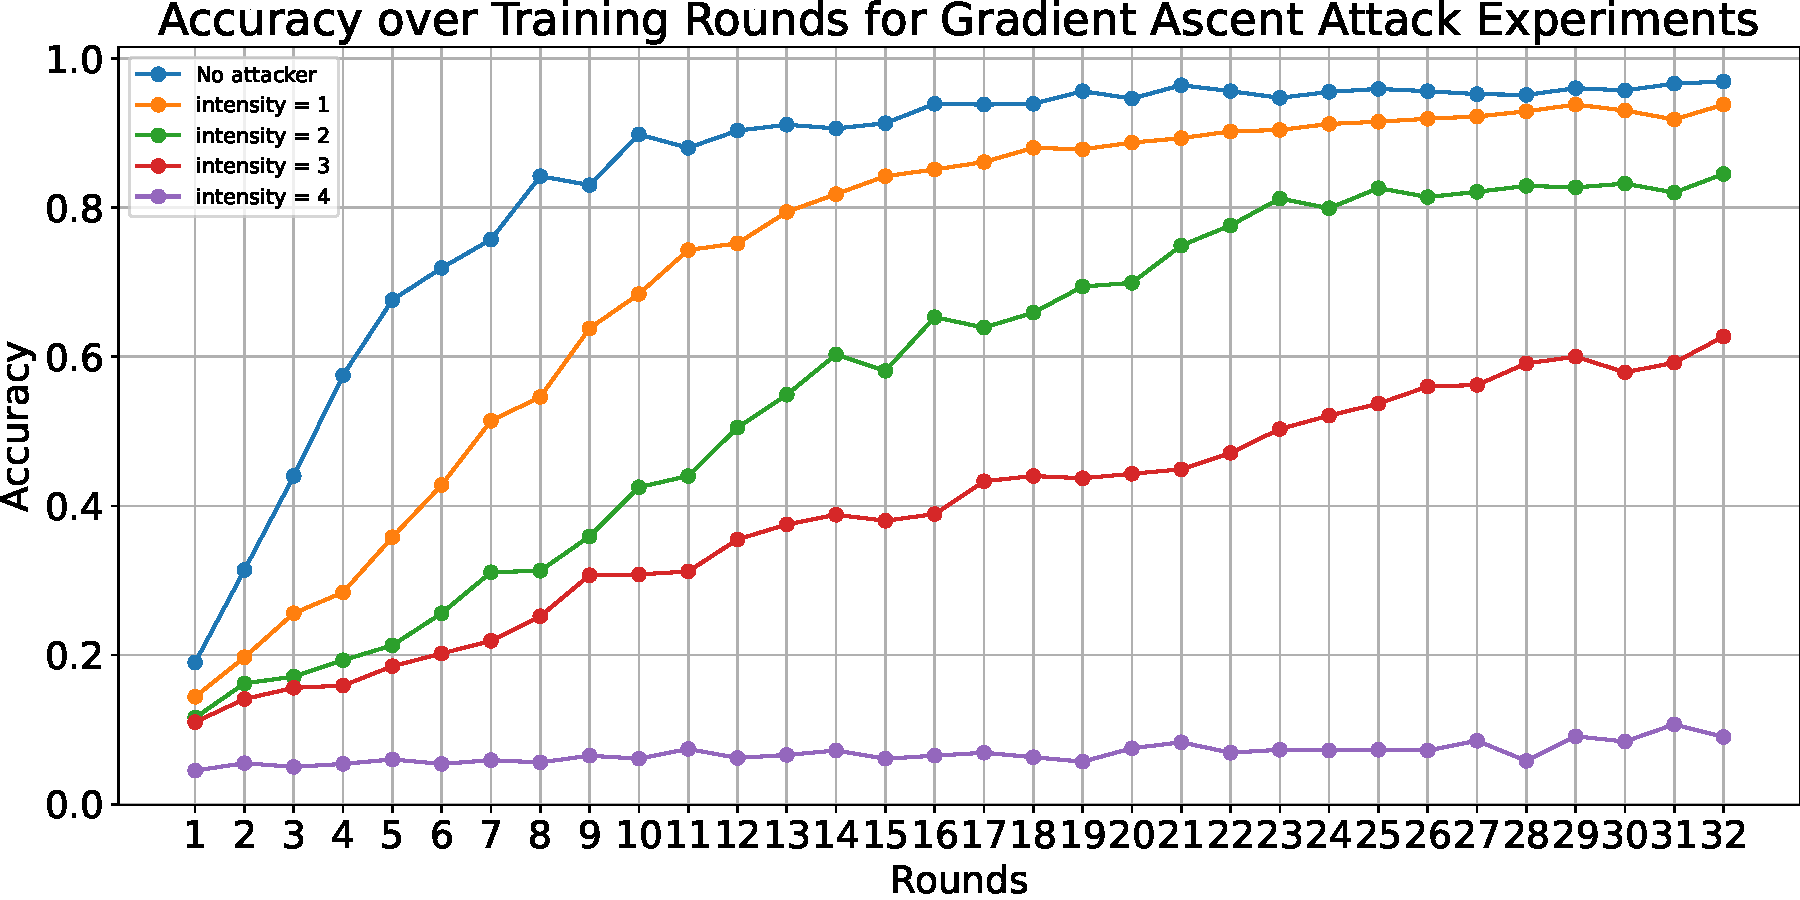
\includegraphics[width=\figGradAscentAttack]{pics/001-gradAttack-attackRate.pdf}}
    % \centering
    % \includesvg[width=0.5\textwidth]{pics/001-gradAttack-attackRate.pdf}
    \caption{grad ascent attack}
    \label{fig:gradAscent}
\end{figure}

We conducted gradient ascent attack experiments on a normal federated learning framework. Without any defense, when 20\% of attackers upload reversed or negatively scaled gradients from their local training, the model accuracy significantly drops. In Figure \hyperref[fig:gradAscent]{\ref{fig:gradAscent}}, the blue curve shows the training accuracy without attackers, while the orange, green, red, and purple curves represent the training results with gradients scaled by $-1$, $-2$, $-3$, and $-4$, respectively. It can be observed that the greater the attack intensity, the more significant the drop in accuracy, indicating the effectiveness of gradient ascent attacks.

% 这是因为,假设每个客户端的数据质量均匀分布、训练效果预期一直,那么每个客户端对于模型准确率的贡献的期望值都是相同的。将这个期望值记为$E$,则正常情况下所有客户端对模型的总贡献期望为$\frac{E\times num}{num}=E$。若其中有$20\%$的客户端将自己的梯度变化量取反,则单个恶意客户端对模型准确率的贡献的期望值是$-E$,所有客户端对模型的总贡献期望为$\frac{E\times num\times(1-20\%)+(-E)\times num\times 20\%}{num} = 0.6E$。同理,若每个客户端将自己的梯度变化量乘以$-2$,则单个客户端的贡献期望为$-2E$,所有客户端贡献总期望为$0.4E$。若单个恶意客户端将自己梯度乘以$-3$,则总贡献期望为$0.2E$。若单个恶意客户端将自己的梯度变化量乘以$-4$,则总贡献期望为$0$。由图\hyperref[fig:gradAscent]{\ref{fig:gradAscent}}所示的对比试验结果可以看出,梯度上升攻击是有效的。

\subsubsection{\textbf{Label Flip Attack}}
\label{exp:attack:label}

\begin{figure}[htbp]
    \centerline{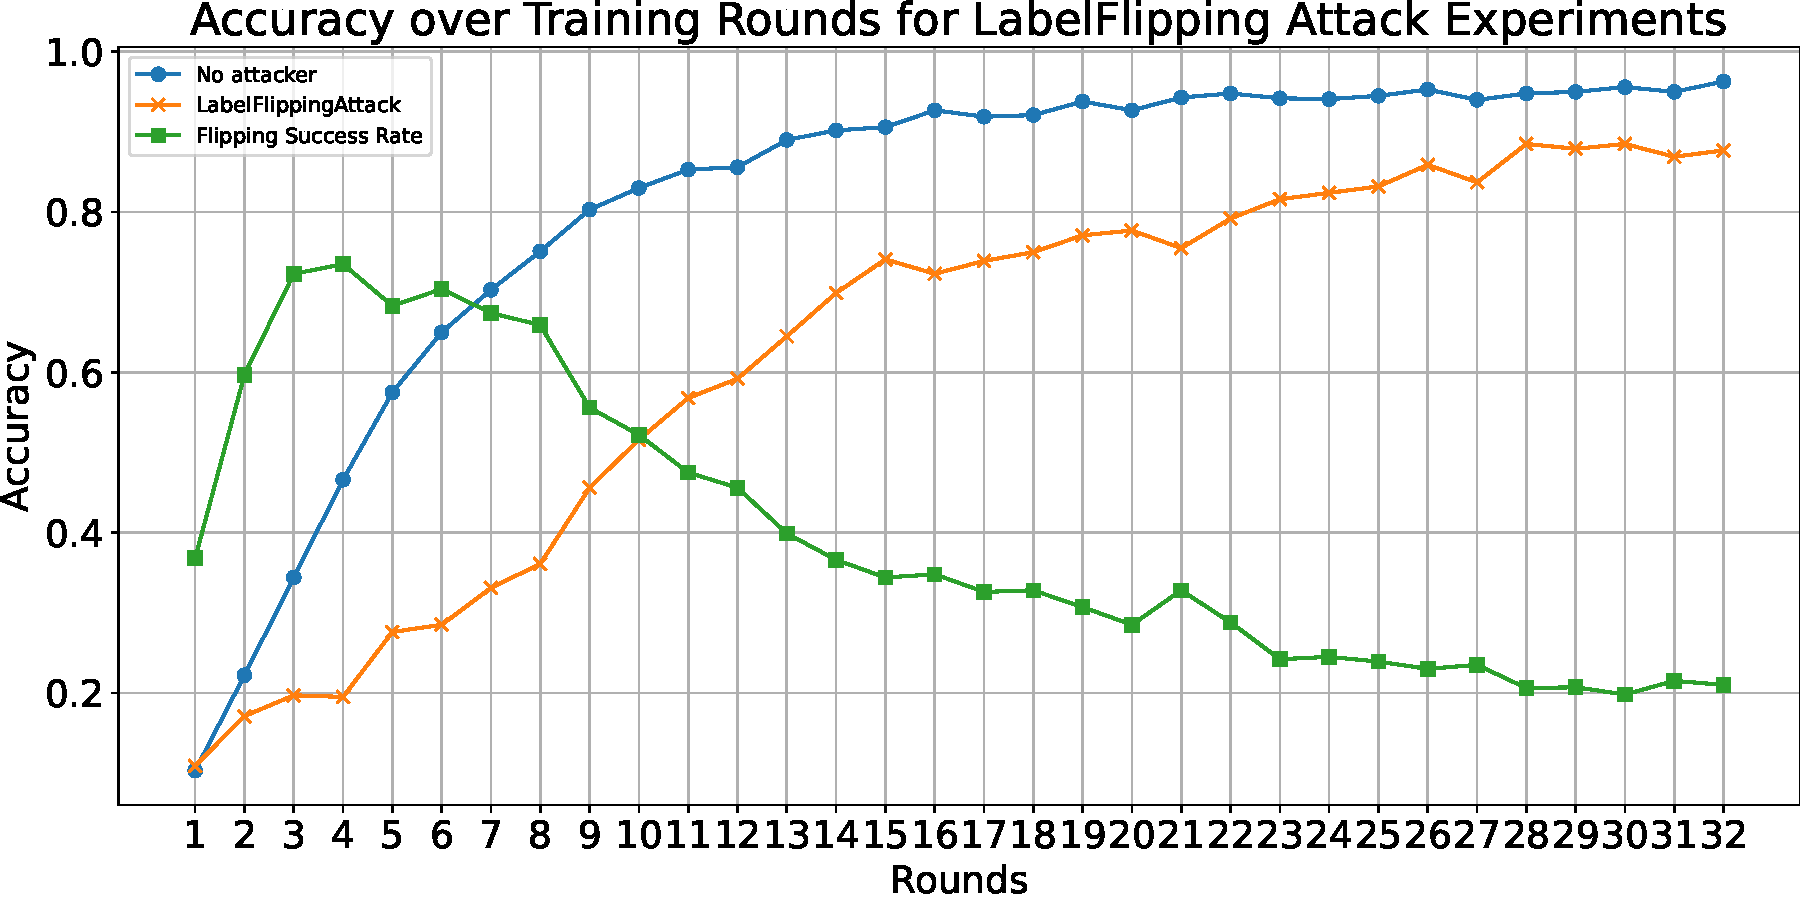
\includegraphics[width=\figLabelFlip]{pics/002-LabelFlippingAttack-attackRate.pdf}}
    \caption{label flip attack}
    \label{fig:labelFlip}
\end{figure}

% 为了验证标签翻转攻击的有效性,我们同样选取$20\%$的客户端作为恶意客户端进行标签翻转攻击,并且不设置防御手段。标签翻转攻击的攻击方式为,篡改本地数据的标签为一个错误的标签。如图\hyperref[fig:labelFlip]{\ref{fig:labelFlip}}所示,蓝色的曲线是没有攻击者时的全局模型准确率变化曲线,橙色的曲线是有$20\%$的恶意客户端进行标签翻转攻击时的准确率变化曲线,而绿色的曲线是标签翻转攻击的成功率曲线,即将图片输入到合并到服务器的全局模型,模型预测结果被误认为攻击目标标签的概率。横坐标表示训练轮次,可以看出,随着训练轮次的增加,标签翻转攻击的成功率首先迅速升高;而随着训练的进行,模型与更多的良性客户端聚合,导致攻击成功率呈现先上升后下降的趋势。标签翻转攻击导致模型的准确率始终不如正常训练的模型准确率,且随着训练轮次的增加,攻击成功率在$20\%$附近维持稳定。实验结果表明,标签反转的攻击也是有效的。

% To verify the effectiveness of label flip attacks, we selected 20\% of the clients as malicious clients to perform label flip attacks without any defense mechanisms. In a label flip attack, the labels of the local data are altered to incorrect labels. As shown in Figure \hyperref[fig:labelFlip]{\ref{fig:labelFlip}}, the blue curve represents the accuracy of the global model without attackers, the orange curve shows the accuracy when 20\% of the clients are performing label flip attacks, and the green curve indicates the success rate of the label flip attack, which is the probability that the global model on the server misclassifies an input image as the attack target label. The x-axis represents the training rounds. It can be seen that as the training rounds increase, the success rate of the label flip attack initially rises quickly; however, as the training progresses, the model aggregates with more benign clients, causing the attack success rate to first increase and then decrease. The label flip attack results in the model's accuracy being consistently lower than that of a normally trained model. With the increase in training rounds, the attack success rate stabilizes around 20\%. The experimental results demonstrate that label flip attacks are also effective.

To verify the effectiveness of label flip attacks, we selected 20\% of clients as malicious and altered the labels of their local data. Figure \hyperref[fig:labelFlip]{\ref{fig:labelFlip}} shows the results: the blue curve represents the global model accuracy without attackers, the orange curve shows the accuracy with 20\% malicious clients, and the green curve indicates the attack success rate, i.e., the probability of the model misclassifying an input image as the target label. Initially, the success rate of the label flip attack rises quickly, but as more benign clients aggregate, it stabilizes around 20%. The model's accuracy remains consistently lower than that of a normally trained model, demonstrating the effectiveness of label flip attacks.

% \subsubsection{\textbf{后门植入攻击}}
\subsubsection{\textbf{Backdoor Attack}}
\label{exp:attack:backdoor}

% 为了验证后门植入攻击的有效性,同样选取$20\%$的客户端作为恶意客户端进行后门植入攻击,且不设置防御手段。每个恶意客户端在本地训练之前,对自己的数据进行后门植入处理,例如将每张图片的左下角3x3的像素点上做标记并更改图片标签。这样在训练过程中,模型会逐渐学习到,当左下角3x3的像素存在标记时,预测结果应该是某个特定的标签。若客户端不进行防御检测,则经过一定轮次的训练后,这一特征就被整合进了全局模型中。当恶意客户端想要让训练好的全局模型将任意一张图片识别为目标标签时,只需要修改这张图片左下角3x3的像素点。这一肉眼难以发现的更改却会导致模型的预测结果发生很大的变化,并带来安全问题。

% To verify the effectiveness of backdoor attacks, we selected 20\% of the clients as malicious clients to perform backdoor attacks without any defense mechanisms. Each malicious client modifies its local data before training by implanting a backdoor, such as marking the bottom-left 3x3 pixels of each image and changing the image label. During training, the model gradually learns that when the bottom-left 3x3 pixels are marked, the prediction should be a specific label. If clients do not conduct defense detection, this feature gets integrated into the global model after several rounds of training. When malicious clients want the trained global model to classify any image as the target label, they only need to modify the bottom-left 3x3 pixels of that image. This subtle change, which is hard to notice with the naked eye, can significantly alter the model's prediction and pose security risks.

To verify the effectiveness of backdoor attacks, we selected 20\% of clients as malicious. These clients modify their local data by implanting a backdoor, such as marking the bottom-left 3x3 pixels of each image and altering the label. During training, the model learns to associate this mark with a specific label. Without defense mechanisms, this feature integrates into the global model, allowing attackers to manipulate the model's predictions by subtly altering images. This poses significant security risks, as the changes are hard to detect visually.

\begin{figure}[htbp]
    \centerline{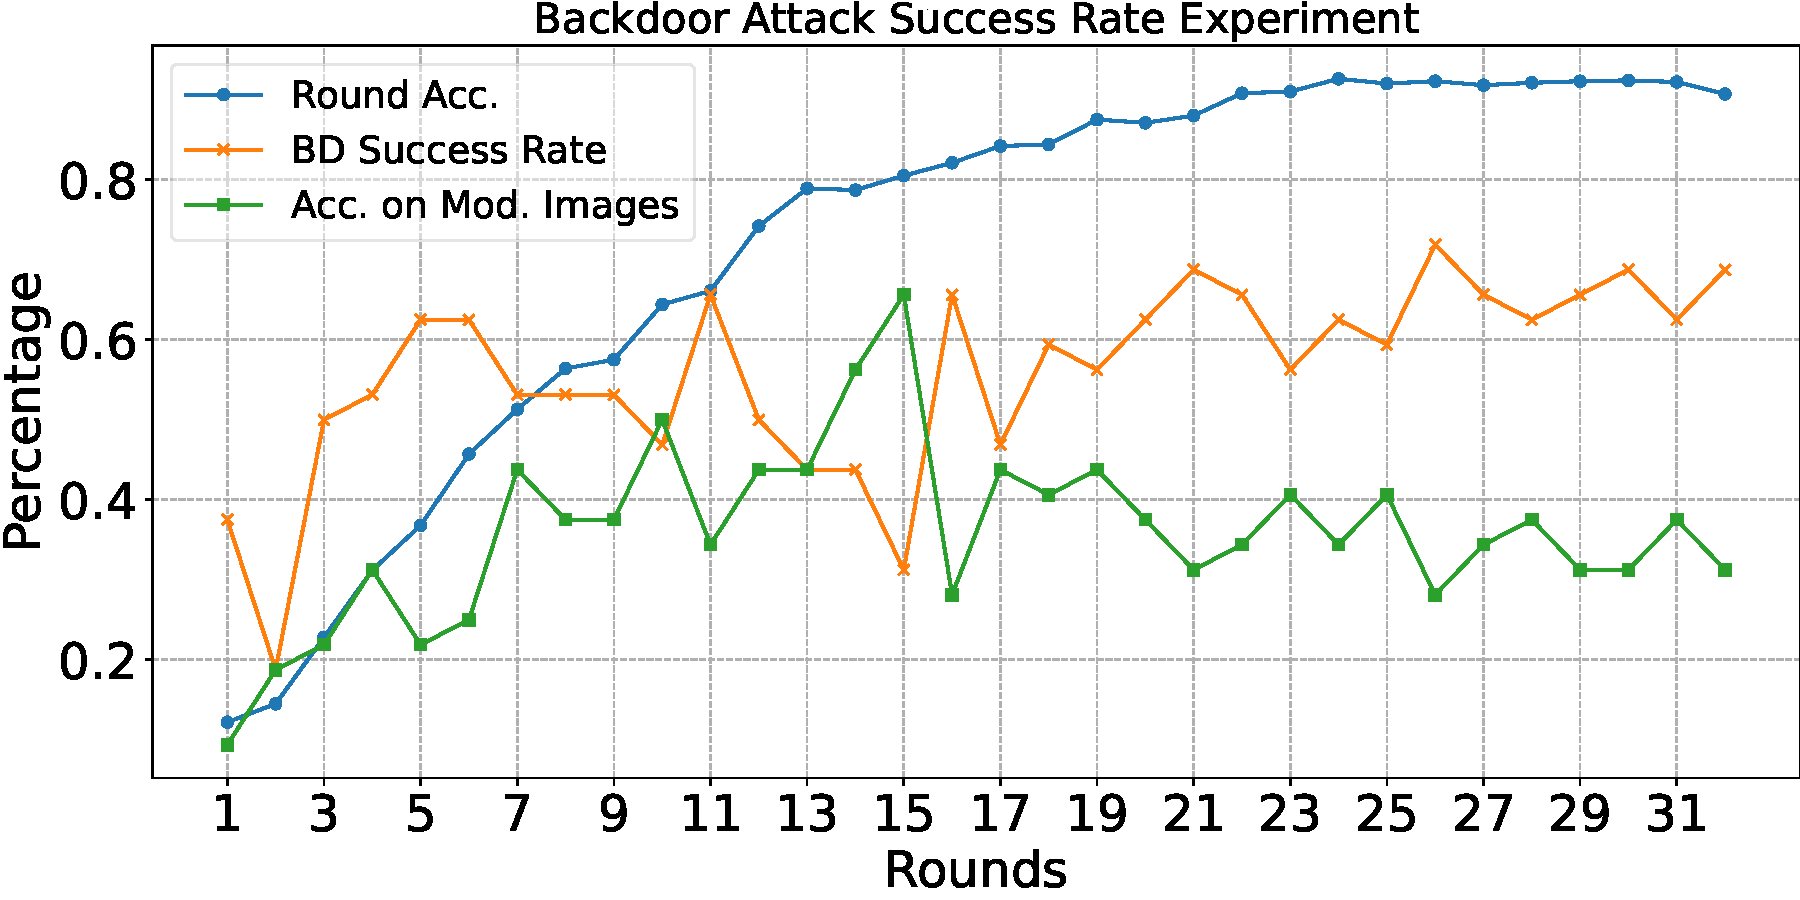
\includegraphics[width=\figBackdoorAttack]{pics/003-backdoorAttack.pdf}}
    % \centering
    % \includesvg[width=0.5\textwidth]{pics/001-gradAttack-attackRate.pdf}
    \caption{backdoor attack}
    \label{fig:backdoorAttack}
\end{figure}

% 图\hyperref[fig:backdoorAttack]{\ref{fig:backdoorAttack}}显示了不加防御的情况下,$20\%$恶意客户端进行上述后门植入攻击的效果。蓝色曲线是模型的准确率曲线,对比图\hyperref[fig:gradAscent]{\ref{fig:gradAscent}}中正常训练的蓝色曲线可以看出,后门攻击十分隐蔽,对模型总的准确率没有太大的影响。由于中央服务器无法预测恶意用户的后门植入方式,因此若不对用户上传的梯度进行检测则很察觉到攻击的发生。图\hyperref[fig:backdoorAttack]{\ref{fig:backdoorAttack}}中橘色曲线显示的是随着轮次的变化,后门植入的成功率。即将多张植入后门的图片输入到全局模型时,模型预测结果为目标标签的概率。可以看出,随着轮次的增加,后门植入的成功率呈现逐渐上升趋势,最高达到了$96.88\%$。图\hyperref[fig:backdoorAttack]{\ref{fig:backdoorAttack}}中绿色的曲线是被篡改的图片的预测准确率,可以看出,随着模型的训练过程,被篡改图片的预测正确率首先呈现逐渐上升的趋势;但是随着训练轮次的增加,后门逐渐被植入到全局模型中,这些图片越来越多地被预测为目标标签。这说明后门攻击也是有效的。

Figure \hyperref[fig:backdoorAttack]{\ref{fig:backdoorAttack}} shows the effect of the backdoor attack conducted by 20\% malicious clients without any defense measures. The blue curve represents the model accuracy. Compared to the normal training blue curve in Figure \hyperref[fig:gradAscent]{\ref{fig:gradAscent}}, it can be seen that the backdoor attack is very stealthy, having little impact on the overall model accuracy. Since the central server cannot predict the backdoor implantation methods of malicious users, it is difficult to detect the attack without examining the uploaded gradients. The orange curve in Figure \hyperref[fig:backdoorAttack]{\ref{fig:backdoorAttack}} shows the success rate of backdoor implantation over training rounds, i.e., the probability that the global model predicts the target label when multiple images with implanted backdoors are input. It can be observed that as the training rounds increase, the success rate of backdoor implantation gradually rises, reaching up to 96.88\%. The green curve indicates the prediction accuracy of the tampered images, showing that the prediction accuracy of the tampered images initially increases with the training process; however, as the training rounds increase, the backdoor gradually gets implanted into the global model, and these images are increasingly predicted as the target label. This indicates that backdoor attacks are also effective.

% 总的来说,实验\hyperref[exp:attack]{\ref{exp:attack}}表明,我们实验中所使用的梯度上升攻击、标签翻转攻击以及后门植入攻击都是有效的。

Overall, the experiments in \hyperref[exp:attack]{\ref{exp:attack}} demonstrate that the gradient ascent attack, label flipping attack, and backdoor implantation attack used in our experiments are all effective.

\subsection{Evaluation of Defense Effectiveness}
\label{exp:defense}

% 在这一部分,我们设计了实验来衡量现有防御方式的防御效果。我们分别使用余弦相似度分析、PCA+余弦相似度分析、特征层提取+PCA+余弦相似度分析、池化放大+PCA+余弦相似度分析;隔离森林、PCA+隔离森林、特征层提取+PCA+隔离森林、池化放大+隔离森林;ViT-MGI等异常检测方式。衡量标准主要有防御准确度和防御速度两个指标。这部分我们选择以CIFAR-10数据集和ViT-B/16模型为例,并分别在ViT-L/16和ViT-H/14模型上、在MNIST和OrganAMNIST数据集上进行验证。



% 余弦相似度分析、PCA+余弦相似度分析、特征层提取+PCA+余弦相似度分析、池化放大+PCA+余弦相似度分析;隔离森林、PCA+隔离森林、特征层提取+PCA+隔离森林、池化放大+隔离森林;ViT-MGI。

% TODO:防御成功性实验:比如进行1000次训练,我们的防御效果。500次在两轮次内全部抓到,...。没有多抓漏抓的情况。

% \subsubsection{\textbf{防御有效性实验}}
\subsubsection{\textbf{Defense Effectiveness Experiment}}
\label{exp:defenseEffectiveness}

% 为了证明我们的防御是有效的,我们在上述三种攻击实验的基础上增加了我们的ViT-MGI防御。

To demonstrate the effectiveness of our defense, we incorporated our ViT-MGI defense into the previously mentioned three attack experiments.

\begin{figure}[htbp]
    \centerline{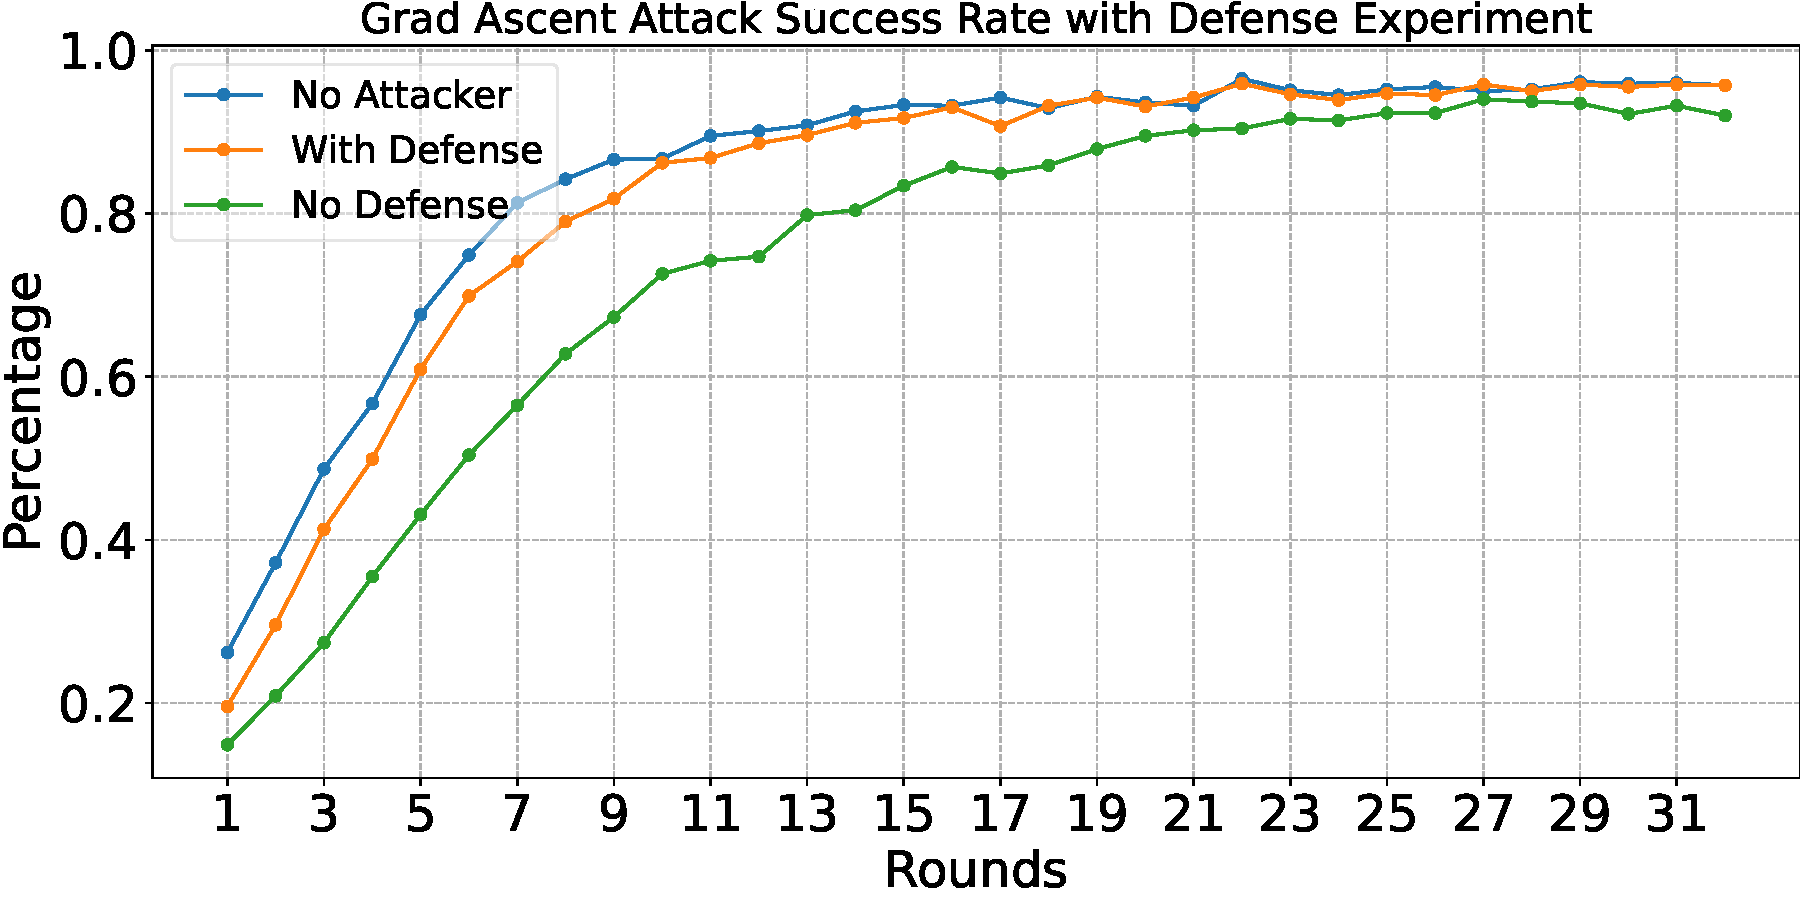
\includegraphics[width=\figGradAscentAttackDefense]{pics/004-gradAttack-attackRate=1-withDefense.pdf}}
    \caption{grad ascent attack and defense}
    \label{fig:gradAscentDefense}
\end{figure}

% 如图\hyperref[fig:gradAscentDefense]{\ref{fig:gradAscentDefense}}所示展示了有$20\%$的恶意客户端进行强度为$1$的梯度上升攻击时的防御效果。蓝色的曲线表示没有攻击者时的准确率随轮次变化的曲线,绿色的表示有攻击者且不进行防御时的准确率变化,而橘色的则表示有攻击者且有ViT-MGI防御时的准确率变化。从图中可以看出,有攻击者而不防御时,模型准确率不如没有攻击者时的准确率。而加上ViT-MGI防御之后,ViT-MGI经过几轮次确定出恶意用户,很快模型的准确率就达到了没有攻击者时候的水平。这说明ViT-MGI是有效的。虽然有攻击但不防御时最终准确率和没有攻击时的差距不是很大,但这是由于攻击强度较低导致的。能够在较低的攻击强度下检测到攻击者并进行防御更能体现ViT-MGI的有效性。

As shown in Figure \hyperref[fig:gradAscentDefense]{\ref{fig:gradAscentDefense}}, we illustrate the defense effect when 20\% of malicious clients perform gradient ascent attacks with a strength of 1. The blue curve represents the accuracy over training rounds with no attackers, the green curve shows the accuracy with attackers but no defense, and the orange curve shows the accuracy with attackers and ViT-MGI defense. The figure demonstrates that with attackers and no defense, the model accuracy is lower than with no attackers. However, with ViT-MGI defense, the model quickly identifies malicious users within a few rounds, and the accuracy soon reaches the level of no attackers. This indicates that ViT-MGI is effective. Although the final accuracy without defense and with attackers is not significantly different from the no-attack scenario, this is due to the low attack strength. Detecting attackers and defending against them at low attack strengths highlights the effectiveness of ViT-MGI.

\begin{figure}[htbp]
    \centerline{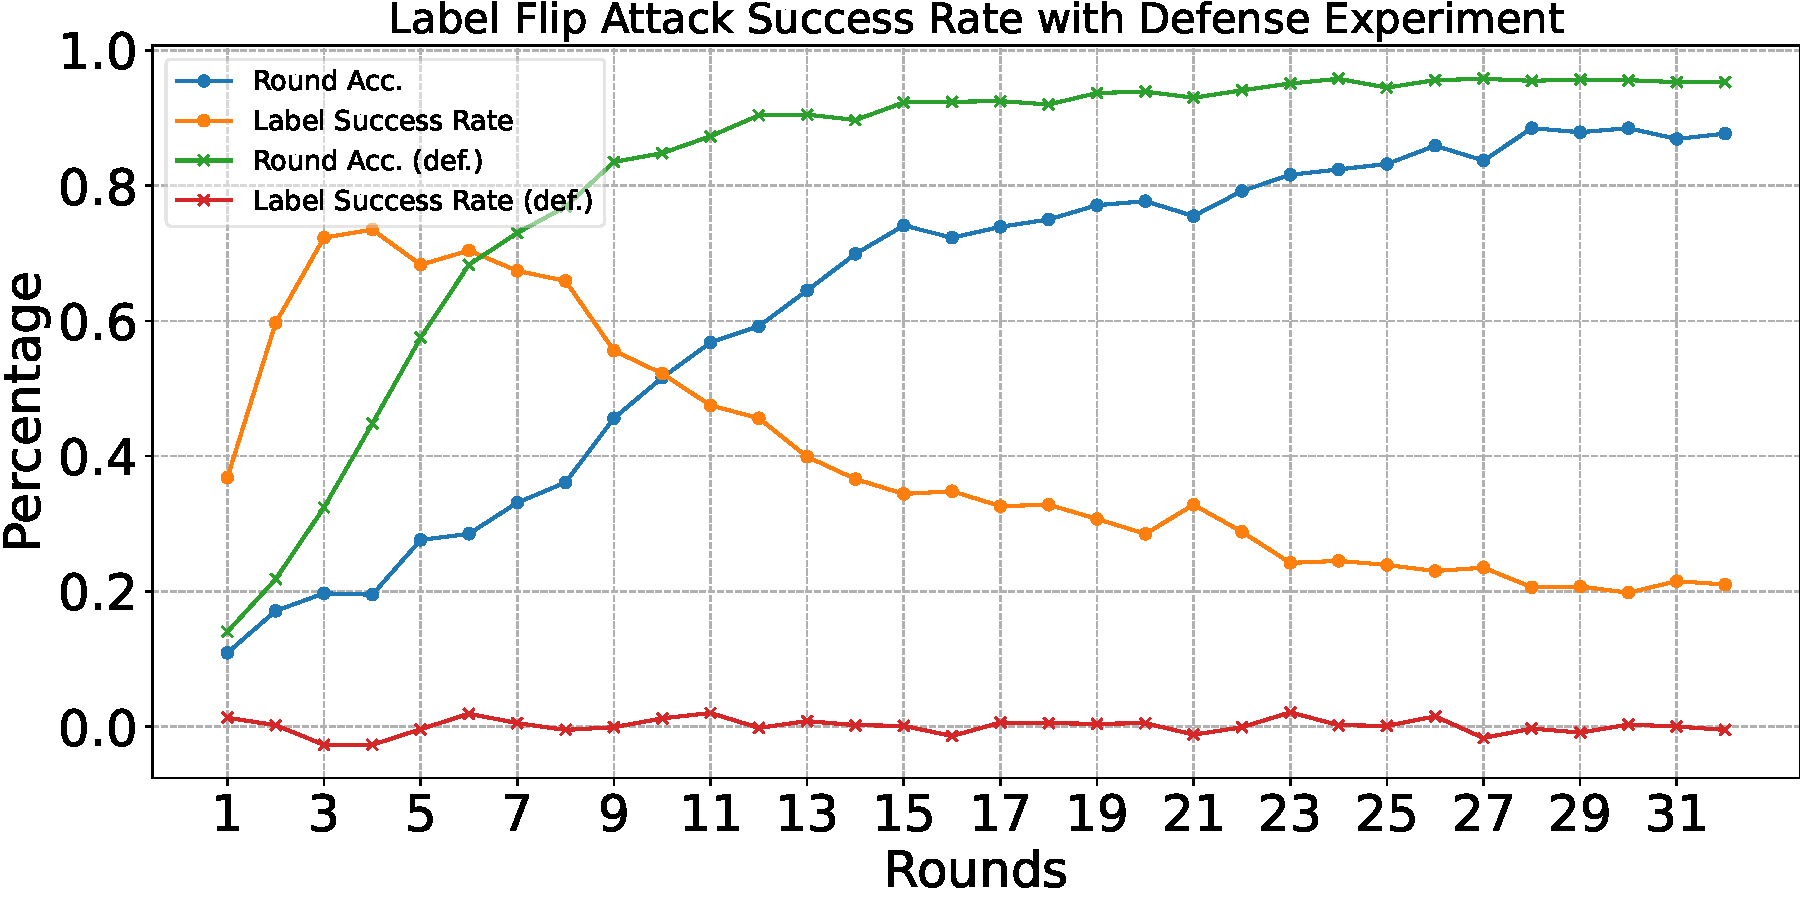
\includegraphics[width=\figLabelFlipDefense]{pics/005-LabelFlippingAttack-withDefense.pdf}}
    \caption{label flipping attack and defense}
    \label{fig:labelFlipDefense}
\end{figure}

% 如图\hyperref[fig:labelFlipDefense]{\ref{fig:labelFlipDefense}}所示展示了有$20\%$的恶意客户端进行标签翻转攻击时的防御效果,攻击方式和\hyperref[exp:attack:label]{\ref{exp:attack:label}}中所描述的一致。蓝色的曲线代表有攻击者但不加防御时的准确率随轮次变化的曲线,绿色的表示有攻击者且加上ViT-MGI防御时的准确率结果。橙色的是没有防御的情况下标签翻转攻击的成功率,而红色的曲线则表示加上ViT-MGI防御时标签翻转攻击成功率。可以看出,若不加防御,标签翻转攻击会导致模型准确率下降,且最终导致有大约$20\%$的标签被错误的识别成目标标签。而加上防御之后,标签攻击的称功率几乎为零,偶尔出现的几个被错误识别成目标标签的情况可能是由模型的总准确率无法达到$100\%$所导致的。这说明ViT-MGI对标签翻转攻击的防御是有效的。

As shown in Figure \hyperref[fig:labelFlipDefense]{\ref{fig:labelFlipDefense}}, we illustrate the defense effect when 20\% of malicious clients perform label-flip attacks, as described in \hyperref[exp:attack:label]{\ref{exp:attack:label}}. The blue curve represents the accuracy over training rounds with attackers but no defense, and the green curve shows the accuracy with attackers and ViT-MGI defense. The orange curve indicates the success rate of the label-flip attack without defense, while the red curve shows the success rate with ViT-MGI defense. The figure demonstrates that without defense, label-flip attacks lead to a decrease in model accuracy and eventually cause about 20\% of the labels to be incorrectly recognized as the target label. However, with ViT-MGI defense, the success rate of label-flip attacks is nearly zero, and the occasional misclassification as the target label is likely due to the model's overall accuracy not reaching 100\%. This indicates that ViT-MGI is effective in defending against label-flip attacks.

\begin{figure}[htbp]
    \centerline{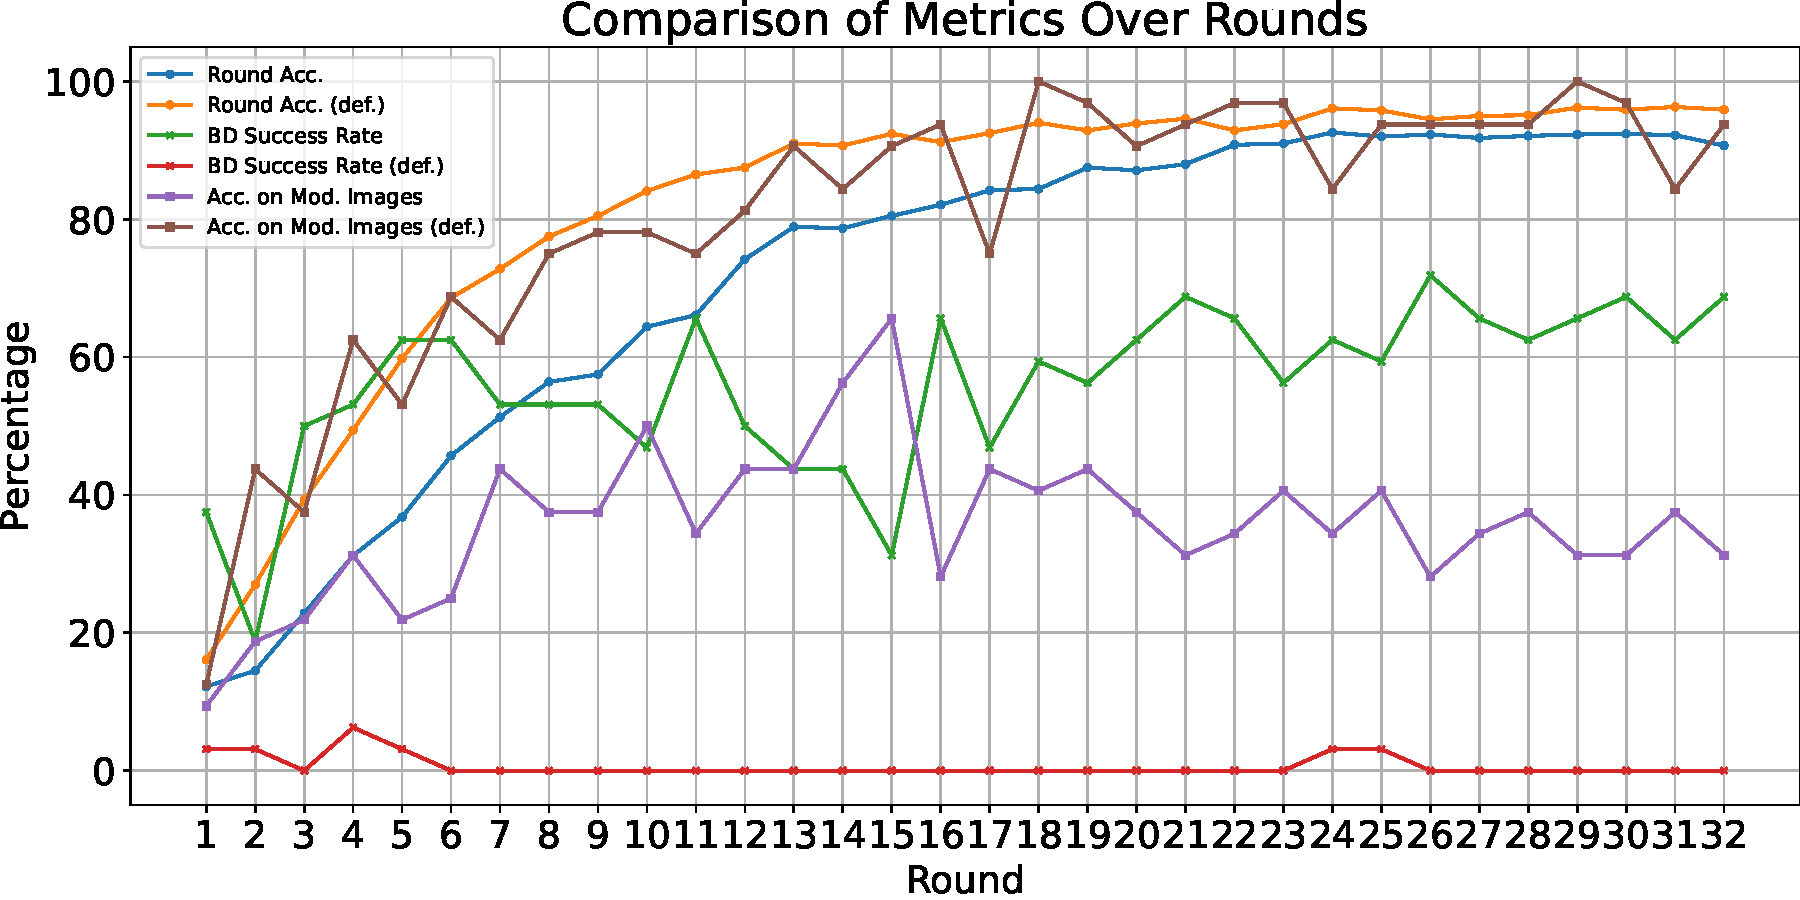
\includegraphics[width=\figBackdoorAttackDefense]{pics/006-backdoorAttack-WithDefense.pdf}}
    \caption{backdoor attack and defense}
    \label{fig:backdoorAttackDefense}
\end{figure}

% 如图\hyperref[fig:backdoorAttackDefense]{\ref{fig:backdoorAttackDefense}}所示展示了有$20\%$的恶意客户端进后门植入攻击时的防御效果,攻击方式和\hyperref[exp:attack:backdoor]{\ref{exp:attack:backdoor}}中所描述的一致。其中蓝色的曲线、绿色的曲线、紫色的曲线分别代表有攻击但没有防御时的模型准确率、后门植入攻击成功率、带有后门的图像的识别准确率;而橙色、红色、棕色的曲线分别代表有防御时的模型准确率、后门植入攻击成功率、带有后门的图像的识别准确率。由紫色曲线和棕色曲线可以看出,后门攻击若不加防御,则对于植入后门的图片的预测准确率很低,而加上ViT-MGI后带有后门的图像的准确率也能接近模型总水平;由绿色曲线和红色曲线能更加清晰地看出ViT-MGI的防御效果,若不加防御则植入后门的图片的成功率能稳定在$70\%$左右,而加上ViT-MGI的防御后植入后门的图片的成功率几乎恒定为$0\%$。这说明ViT-MGI对后门植入攻击的防御是有效的。

% As shown in Figure \hyperref[fig:backdoorAttackDefense]{\ref{fig:backdoorAttackDefense}}, we present the defense effect when 20\% of malicious clients perform backdoor attacks, as described in \hyperref[exp:attack:backdoor]{\ref{exp:attack:backdoor}}. The blue, green, and purple curves represent the model's accuracy, backdoor attack success rate, and the recognition accuracy of images with backdoors when there are attacks but no defense, respectively. The orange, red, and brown curves represent the model's accuracy, backdoor attack success rate, and the recognition accuracy of images with backdoors when ViT-MGI defense is applied. From the purple and brown curves, it can be observed that without defense, the prediction accuracy for images with backdoors is very low, whereas with ViT-MGI, the accuracy for images with backdoors can approach the overall model level. The green and red curves more clearly demonstrate the effectiveness of ViT-MGI defense. Without defense, the success rate of backdoor images remains stable at around 70\%, while with ViT-MGI defense, the success rate of backdoor images is nearly 0\%. This indicates that ViT-MGI is effective in defending against backdoor attacks.

Figure \hyperref[fig:backdoorAttackDefense]{\ref{fig:backdoorAttackDefense}} shows the defense effect when 20\% of malicious clients perform backdoor attacks. The blue, green, and purple curves represent the model's accuracy, backdoor attack success rate, and the recognition accuracy of images with backdoors without defense, respectively. The orange, red, and brown curves represent the same metrics when ViT-MGI defense is applied. Without defense, the recognition accuracy for backdoor images is very low, while with ViT-MGI, the accuracy approaches the overall model level. The green and red curves demonstrate that without defense, the success rate of backdoor attacks remains around 70\%, but with ViT-MGI, the success rate drops to nearly 0\%, indicating the effectiveness of ViT-MGI against backdoor attacks.

% \subsubsection{\textbf{防御准确度衡量}}
\subsubsection{\textbf{Defense Accuracy Measurement}}
\label{exp:defense_accuracy}

% 对于恶意用户的攻防,我们使用以下指标来衡量不同算法的性能:

To evaluate the effectiveness of defense mechanisms against malicious clients, we use the following metrics to measure the performance of different algorithms:

% 1. TP(True Positives,真正例): 被正确识别为恶意客户端的恶意客户端数量。
% 2. TN(True Negatives,真负例): 被正确识别为正常客户端的正常客户端数量。
% 3. FP(False Positives,假正例): 被错误识别为恶意客户端的正常客户端数量。
% 4. FN(False Negatives,假负例): 被错误识别为正常客户端的恶意客户端数量。

1. TP (True Positives): The number of malicious clients correctly identified as malicious.
2. TN (True Negatives): The number of normal clients correctly identified as normal.
3. FP (False Positives): The number of normal clients incorrectly identified as malicious.
4. FN (False Negatives): The number of malicious clients incorrectly identified as normal.


% % 1. 精确率 (Precision): 精确率衡量的是被识别为恶意客户端中实际为恶意客户端的比例。
% 1. Precision: Precision measures the proportion of clients identified as malicious that are actually malicious.
%     \[
%     \text{Precision} = \frac{TP}{TP + FP}
%     \]

% % 2. 召回率 (Recall): 召回率衡量的是实际恶意客户端中被正确识别的比例。
% 2. Recall: Recall measures the proportion of actual malicious clients that are correctly identified.
%     \[
%     \text{Recall} = \frac{TP}{TP + FN}
%     \]

% % 3. F1分数 (F1 Score): F1分数是精确率和召回率的调和平均值,综合考虑了两者的表现。
% 3. F1 Score: The F1 Score is the harmonic mean of precision and recall, providing a balance between the two.
%     \[
%     \text{F1 Score} = \frac{2 \times \text{Precision} \times \text{Recall}}{\text{Precision} + \text{Recall}}
%     \]

% % 4. 准确率 (Accuracy): 准确率衡量的是所有客户端中被正确识别的比例。
% 4. Accuracy: Accuracy measures the proportion of all clients that are correctly identified.
%     \[
%     \text{Accuracy} = \frac{TP + TN}{TP + TN + FP + FN}
%     \]

% 4. 假阳性率 (False Positive Rate, FPR): 假阳性率衡量的是实际正常客户端中被错误识别为恶意客户端的比例。
%     \[
%     \text{FPR} = \frac{FP}{FP + TN}
%     \]

% 5. 假阴性率 (False Negative Rate, FNR): 假阴性率衡量的是实际恶意客户端中被错误识别为正常客户端的比例。
%     \[
%     \text{FNR} = \frac{FN}{TP + FN}
%     \]

% 7. ROC曲线 (ROC Curve): ROC曲线是以假阳性率为横轴,真阳性率(即召回率)为纵轴绘制的曲线,用来评价分类器的性能。
%     - AUC值 (Area Under Curve): AUC值是ROC曲线下的面积,数值越接近1,说明分类器性能越好。

% 由图\hyperref[fig:backdoorAttack]{\ref{fig:backdoorAttack}}可以看出,后门植入攻击能够在几乎不影响模型准确率的情况下进行,其十分难以被察觉。随着时间的推移,可能会出现越来越多的新型攻击方式,其同样很难被发掘。

% 对于梯度上升攻击,攻击者梯度乘以的倍率的绝对值越大则攻击效果越好;对于标签翻转攻击和后门植入攻击,篡改的数据集比例越大则攻击效果越好;但攻击效果更好的同时就越容易被检测出来。对于恶意客户端的比例,更大的攻击者占比会导致更难被算法识别。

% \begin{table}[htbp]
%     \caption{Grad Ascent Defense Result}
%     \begin{center}
%     \begin{tabular}{|c|c|c|c|c|c|}
%     \hline
%     \textbf{Defend Method} & \textbf{Recall} & \textbf{Precision} & \textbf{F1 Score} & \textbf{Accuracy} & \textbf{Time(s)} \\
%     \hline 
%     \textbf{Head} & \textbf{\textit{Table column subhead}}& \textbf{\textit{Subhead}}& \textbf{\textit{Subhead}} \\
%     \hline
%     copy& More table copy$^{\mathrm{a}}$& &  \\
%     \hline
%     \end{tabular}
%     \label{tab1}
%     \end{center}
% \end{table}

\begin{table}[htbp]
    \caption{Grad Ascent Defense Result}
    % \vspace{-10pt}  % 这个是我加的,要不然标头与表格离得太远了
    \begin{center}
    \resizebox{\linewidth}{!}{
    \begin{tabular}{|c|c|c|c|c|c|}
    \hline
    \textbf{Defend Method} & \textbf{Recall} & \textbf{Precision} & \textbf{F1 Score} & \textbf{Accuracy} & \textbf{Time(s)} \\
    \Xhline{3\arrayrulewidth}
    Both-layer & 1.0 & 1.0 & 1.0 & 1.0 & 261 \\
    \hline
    Both-only & 0.992 & 1.0 & 0.996 & 0.994 & 1012 \\
    \hline
    Both-pooling & 0.992 & 0.996 & 0.994 & 0.991 & 605 \\
    \Xhline{3\arrayrulewidth}
    PCA-layer & 0.988 & 0.969 & 0.978 & 0.966 & 307 \\
    \hline
    PCA-only & 0.98 & 0.951 & 0.965 & 0.944 & 991 \\
    \hline
    PCA-pooling & 0.961 & 0.904 & 0.932 & 0.887 & 593 \\
    \Xhline{3\arrayrulewidth}
    Forest-layer & 0.984 & 0.86 & 0.918 & 0.859 & 463 \\
    \hline
    Forest-pooling & 0.922 & 0.814 & 0.865 & 0.769 & 313 \\
    \hline
    \end{tabular}}
    \label{tab:gradAscent}
    \end{center}
\end{table}

% 表\hyperref[tab:gradAscent]{\ref{tab:gradAscent}}展示了各种防御算法针对梯度上升攻击的恶意客户端识别结果。其中Defend Method中,hyphen前代表防御方式,hyphen后代表数据降维方式。其中hyphen前有PCA、Forest、以及Both三种,PCA代表主成分分析加余弦相似度检测,Forest代表隔离森林检测,Both代表ViT-MGI中使用的先进行主成分分析再进行隔离森林的检测方式;而hyphen后有layer、pooling以及only三种,分别代表通过提取特征层的方式、放大池化的方式以及不进行数据提取操作者三种方式。若参数量较大的ViT模型直接应用隔离森林算法,则会造成大量的时间及内存消耗($> 128GB$),因此面对数据量较大的ViT模型时,有理由认为单纯的隔离森林不是一种有效的防御检测方法。

% 不论是使用PCA+余弦相似度检测还是使用PCA+隔离森林,可以发现最近提出的放大池化\cite{betterTogether}算法在面对数据量较大的ViT模型时,会导致识别效果变差,而使用我们发现的特征层提取算法都能提升识别准确度。

% Table \hyperref[tab:gradAscent]{\ref{tab:gradAscent}} presents the results of various defense algorithms in identifying malicious clients under gradient ascent attacks. In the Defend Method column, the part before the hyphen represents the defense method, and the part after the hyphen represents the data dimensionality reduction method. There are three defense methods: PCA, Forest, and Both. PCA stands for principal component analysis combined with cosine similarity detection, Forest stands for isolation forest detection, and Both represents the ViT-MGI method, which first performs principal component analysis followed by isolation forest detection. The data reduction methods are layer, pooling, and only, representing feature layer extraction, pooling amplification, and no data extraction, respectively. Applying the isolation forest algorithm directly to a ViT model with a large number of parameters results in significant time and memory consumption (greater than 128GB). Therefore, it is reasonable to consider that isolation forest alone is not an effective defense detection method for large ViT models.

% Whether using PCA with cosine similarity detection or PCA with isolation forest, the recently proposed pooling amplification algorithm \cite{betterTogether} shows degraded detection performance with large ViT models. However, using our feature layer extraction method improves detection accuracy.


Table \hyperref[tab:gradAscent]{\ref{tab:gradAscent}} shows the performance of various defense algorithms against gradient ascent attacks. The Defend Method column lists the defense method and the data dimensionality reduction method. The defense methods include PCA (principal component analysis with cosine similarity detection), Forest (isolation forest detection), and Both (ViT-MGI, combining PCA with isolation forest). The data reduction methods are layer (feature layer extraction), pooling (pooling amplification), and only (no data extraction).

Applying isolation forest directly to large ViT models is impractical due to significant time and memory consumption (>128GB). Hence, isolation forest alone is not effective for large ViT models.

Both PCA with cosine similarity detection and PCA with isolation forest show that the pooling amplification algorithm \cite{betterTogether} degrades detection performance in large ViT models. However, our feature layer extraction method significantly improves detection accuracy.

\begin{table}[htbp]
    \caption{Grad Ascent Defense Result}
    % \vspace{-10pt} % 减少标题和表格之间的间距
    \begin{center}
    \resizebox{\linewidth}{!}{
    \begin{tabular}{|c|c|c|c|c|c|}
    \hline
    \textbf{Defend Method} & \textbf{Recall} & \textbf{Precision} & \textbf{F1 Score} & \textbf{Accuracy} & \textbf{Time(s)} \\
    \Xhline{3\arrayrulewidth}
    Both-layer & 0.991 & 1.0 & 0.995 & 0.994 & 273 \\
    \hline
    Both-only & 0.991 & 1.0 & 0.995 & 0.994 & 964 \\
    \hline
    Both-pooling & 0.987 & 0.974 & 0.98 & 0.972 & 579 \\
    \Xhline{3\arrayrulewidth}
    PCA-layer & 1.0 & 0.896 & 0.945 & 0.919 & 346 \\
    \hline
    PCA-only & 0.987 & 0.867 & 0.923 & 0.884 & 1017 \\
    \hline
    PCA-pooling & 0.955 & 0.823 & 0.884 & 0.825 & 608 \\
    \Xhline{3\arrayrulewidth}
    Forest-layer & 0.991 & 0.844 & 0.912 & 0.866 & 472 \\
    \hline
    Forest-pooling & 0.973 & 0.829 & 0.895 & 0.841 & 327 \\
    \hline
    \end{tabular}}
    \label{tab:labelFlip}
    \end{center}
\end{table}

\begin{table}[htbp]
    \caption{Grad Ascent Defense Result}
    % \vspace{-10pt} % 减少标题和表格之间的间距
    \begin{center}
    \resizebox{\linewidth}{!}{
    \begin{tabular}{|c|c|c|c|c|c|}
    \hline
    \textbf{Defend Method} & \textbf{Recall} & \textbf{Precision} & \textbf{F1 Score} & \textbf{Accuracy} & \textbf{Time(s)} \\
    \Xhline{3\arrayrulewidth}
    Both-layer & 0.969 & 0.995 & 0.982 & 0.975 & 269 \\
    \hline
    Both-only & 0.982 & 0.952 & 0.967 & 0.953 & 1041 \\
    \hline
    Both-pooling & 0.955 & 0.982 & 0.968 & 0.956 & 623 \\
    \Xhline{3\arrayrulewidth}
    PCA-layer & 0.996 & 0.861 & 0.924 & 0.884 & 316 \\
    \hline
    PCA-only & 0.987 & 0.847 & 0.912 & 0.866 & 955 \\
    \hline
    PCA-pooling & 0.991 & 0.838 & 0.908 & 0.859 & 586 \\
    \Xhline{3\arrayrulewidth}
    Forest-layer & 0.996 & 0.772 & 0.87 & 0.791 & 471 \\
    \hline
    Forest-pooling & 0.951 & 0.801 & 0.87 & 0.8 & 352 \\
    \hline
    \end{tabular}}
    \label{tab:backdoor}
    \end{center}
\end{table}

% 表\hyperref[tab:labelFlip]{\ref{tab:labelFlip}}和表\hyperref[tab:backdoor]{\ref{tab:backdoor}}分别表示了标签翻转攻击和后门植入攻击时的各种算法防御效果对比,其中标签翻转攻击以及后门植入攻击都有$30\%$的攻击者,其中后门植入攻击的攻击者只将本地$35\%$的数据进行了后门植入处理。结果发现,和表\hyperref[tab:gradAscent]{\ref{tab:gradAscent}}的结果类似,放大池化算法都在降低计算量的同时降低了识别精度。而我们的特征层提取算法能够在降低计算量的同时聚合有效信息,使得后续计算效果更加准确。

% Tables \hyperref[tab:labelFlip]{\ref{tab:labelFlip}} and \hyperref[tab:backdoor]{\ref{tab:backdoor}} respectively present the defense effectiveness of various algorithms against label-flipping attacks and backdoor attacks. Both the label-flipping attack and the backdoor attack scenarios involve $30\%$ malicious clients, with the backdoor attackers embedding backdoors in only $35\%$ of their local data. The results indicate that, similar to the findings in Table \hyperref[tab:gradAscent]{\ref{tab:gradAscent}}, the pooling amplification algorithm reduces computational load but also decreases detection accuracy. In contrast, our feature layer extraction method not only reduces computational load but also aggregates valuable information, thereby enhancing the accuracy of subsequent calculations.

Tables \hyperref[tab:labelFlip]{\ref{tab:labelFlip}} and \hyperref[tab:backdoor]{\ref{tab:backdoor}} show the effectiveness of various defense algorithms against label-flipping and backdoor attacks, respectively. Both scenarios involve $30\%$ malicious clients, with backdoor attackers embedding backdoors in $35\%$ of their local data. Similar to the findings in Table \hyperref[tab:gradAscent]{\ref{tab:gradAscent}}, the pooling amplification algorithm reduces computational load but decreases detection accuracy. In contrast, our feature layer extraction method not only reduces computational load but also enhances accuracy by aggregating valuable information.

% \subsubsection{\textbf{防御速度衡量}}
\subsubsection{\textbf{Defense Speed Measurement}}

% 由不进行数据降维的两个实验可以看出,不论使用何种算法都会消耗大量的时间,这对于平均耗时只有165秒的训练过程来说是无法接受的。

% 我们在相同环境、相同训练参数的情况下分别进行了上述实验,并统计了正常训练耗时、以及应用上各种防御方式后的总耗时。由表\hyperref[tab:gradAscent]{\ref{tab:gradAscent}}-表\hyperref[tab:backdoor]{\ref{tab:backdoor}}可以看出,我们的方案在效率和鲁棒性方面都有更好的表现。

From the experiments where no data dimensionality reduction was performed, it is evident that regardless of the algorithm used, a substantial amount of time is consumed, which is unacceptable for a training process that typically takes only 165 seconds on average.

We conducted the aforementioned experiments under the same environment and training parameters and recorded the normal training time and the total time with various defense methods applied. As shown in Tables \hyperref[tab:gradAscent]{\ref{tab:gradAscent}} through \hyperref[tab:backdoor]{\ref{tab:backdoor}}, our approach demonstrates superior performance in both efficiency and robustness.

% \subsection{特征层确定}
\subsection{Feature Layer Determination}
\label{exp:exp_layer}

% 为了减小恶意攻击检测所需要的计算量以及剔除对恶意用户检测不是那么有效的数据,我们进行了一系列待提取特征层的确定实验。实验方法并不困难,对于某种攻击,我们可以将这个攻击的所有层全部提取出来,对于每一层,ViT-MGI中除了特征层提取部分的防御方法进行防御,只挑选防御效果特别好的层。这样,对于一种攻击方式,我们就能得到一些候选的待提取特征层,将多种攻击所得到的层进行求交集运算,即能得对所有攻击都很敏感的层。多次进行上述实验,将每次的实验结果进行求和累计,统计每个层在多次实验中的候选次数。最后,我们对这些层按照候选总次数进行由高到低的排序,即能得到对于攻击十分敏感的层。算法的伪代码如\hyperref[alg:featureLayerSelection]{Algorithm \ref{alg:featureLayerSelection}}所示。

To reduce the computational load required for detecting malicious attacks and to eliminate data that is not effective for detecting malicious users, we conducted a series of experiments to determine the feature layers to be extracted. The experimental method is straightforward: for a specific attack, we extract all layers associated with this attack, and for each layer, we apply ViT-MGI's defense methods excluding the feature layer extraction part, selecting only the layers that show particularly good defense effects. In this way, for each type of attack, we obtain several candidate feature layers. By finding the intersection of the layers obtained from multiple types of attacks, we identify layers that are sensitive to all attacks. Repeating these experiments multiple times and accumulating the results, we count the number of times each layer appears as a candidate. Finally, we sort these layers by the total number of times they appear as candidates, in descending order, to identify the layers that are highly sensitive to attacks. The pseudocode for the algorithm is shown in\hyperref[alg:featureLayerSelection]{Algorithm \ref{alg:featureLayerSelection}}.

% \begin{algorithm}
%     \caption{Feature Layer Selection Experiment for Reducing Computational Cost of Malicious Attack Detection}
%     \label{alg:featureLayerSelection}
%     \begin{algorithmic}[1]
%     \State Initialize candidate\_layers as an empty set
    
%     \For{each attack in attack\_methods}
%         \State Extract all layers for the given attack
%         \State Initialize defense\_effectiveness as an empty set
    
%         \For{each layer in all\_layers}
%             \State Apply ViT-MGI defense method (excluding feature layer extraction part)
%             \State Record defense effectiveness in defense\_effectiveness[layer]
%         \EndFor
    
%         \State Select layers with the best defense effectiveness
%         \For{each layer in selected\_layers}
%             \If{layer not in candidate\_layers}
%                 \State candidate\_layers[layer] = 0
%             \EndIf
%             \State candidate\_layers[layer] += 1
%         \EndFor
%     \EndFor
    
%     \State Find intersection of layers sensitive to all attacks as sensitive\_layers
    
%     \For{each experiment in multiple\_experiments}
%         \State result = conduct\_experiment(experiment)
%         \For{each layer in result}
%             \If{layer not in candidate\_layers}
%                 \State candidate\_layers[layer] = 0
%             \EndIf
%             \State candidate\_layers[layer] += 1
%         \EndFor
%     \EndFor
    
%     \State Sort sensitive layers by total candidate count as sorted\_sensitive\_layers
    
%     \State Extract and integrate gradients of sensitive layers for malicious user detection
    
%     \State Randomly select additional layers from non-extracted layers for integration to prevent targeted attacks
%     \end{algorithmic}
% \end{algorithm}


\begin{algorithm}
    \caption{Feature Layer Selection and Integration}
    \label{alg:featureLayerSelection}
    \begin{algorithmic}[1]
        \Require $A$ - List of attack methods, $G$ - Gradients uploaded by malicious users each time
        \Ensure $I$ - Integrated gradients for defense detection

        \Function{FeatureSelect}{$A, G$}
            \State $C \gets \left [ \right ] $
            \For{each $G_i$ in $G$}
                \State $C.append( \Call{SelectOnce}{A, G_i})$
            \EndFor
            \State $T \gets CountTimes(C)$
            \State $SortByTimes(T)$
            \State $I, times \gets getHighTimes(T)$
            \State \Return $I$
        \EndFunction

        \Function{SelectOnce}{$A, G_i$}
            \State $S \gets \left [  \right ] $
            \For{each $a$ in $A$}
                \State $L \gets$ extract all layers from $G_i$
                \State $S_a \gets \emptyset$
                \For{each $l$ in $L$}
                    \State $acc_l \gets MGI(l)$
                    \If{$acc_l = 100\%$}
                        \State $S.insert(l)$
                    \EndIf
                \EndFor
            \State $C \gets \bigcap\left \{ s | s\in S  \right \}$
            \EndFor
            \State \Return $C$
        \EndFunction

        % \Function{Extract}{$g, L_k$}
        %     \State $\phi(g) \gets \emptyset$
        %     \For{each $l$ in $g.layers()$}
        %         \If{$l.name \in L_k$}
        %             \State $\phi(g) \gets \phi(g) + l$
        %         \EndIf
        %     \EndFor
        %     \State \Return $\phi(g)$
        % \EndFunction

        

        % \State $L_s \gets \Call{FeatureSelect}{A}$
        % \State $I_g \gets \Call{Integrate}{G, L_s}$

    \end{algorithmic}
\end{algorithm}

% 这样,对于恶意用户上传的梯度,我们就可以只提取这些层的梯度后整合到一起,再进行后续的防御检测。为了防止恶意用户针对本算法进行攻击,可以每次随机选取一些在提取名单之外的层进行整合。% \footnote{忽然想到针对候选的每一层做一个识别实验,将所有层的结果按出现次数排序不知道会咋样。}

Thus, for the gradients uploaded by malicious users, we can extract only the gradients of these identified layers, integrate them, and then proceed with subsequent defense detection. To prevent malicious users from attacking this algorithm specifically, we can randomly select some layers outside the extraction list for integration each time.

% Experiments:

% 实验设置(用的xx机器,在xx跑,用的xx模型xx参数,对比的哪些攻击/防御,数据集,...)能一大段

% 实验结果分析(分点)

% 比如:
% 1. 精度
% 2. 速度
% 3. 防御效果
% 对比着给点结论。

% \textcolor{red}{一直跑着实验}
% (最好写的部分)





\section{Conclusion}
\label{sec:conclusion}
% 单独PCA太慢又不准,单独隔离森林纯乱抓(因为无效数据太多了),池化(最大池、平均池)+PCA、池化+隔离森林都只能提升计算效率,但是准确率会下降很多。

% 最终发现提取特征层后,先进行PCA降维,再进行隔离森林,结合上主观逻辑模型,效果最好。

% 单独的提取特征层+PCA降维+隔离森林就已经很不错了,基本上每次都会抓对。(恶意攻击被识别的准确率几乎100\%),单看某次来说可能会抓一两个无辜的,但是无辜用户被抓地很随机,结合上主观逻辑模型几轮次下来几乎就能确定出来了。

% 实验结果表明,在检测恶意用户的拜占庭攻击时,若单独使用主成分分析算法,则耗时较长且检测结果不准确,无法应用到实际的项目中去。若单独使用隔离森林算法则因大量参数中包含着大量的对恶意检测无效的数据,导致检测准确性极低,甚至接近随机抓取的效果。若使用池化技术\cite{betterTogether}对数据进行降维后再进行PCA提取异常成分,则仅仅会减少PCA的时间损耗而会导致检测准确性降低。使用池化技术加上隔离森林算法则同样如此,只能减少计算耗时而无法提升检测准确率。最终发现,拜占庭攻击发生时由于ViT每层的敏感程度不同,所以可以先通过提取特征层的方式,降低数据量的同时去除对异常检测无效的数据,再通过PCA降维聚类,聚合提取异常数据,最后通过隔离森林算法进行检测,实现效果最好。这种方法的恶意攻击检测准确率几乎达到100\%,对于较低的误报率而言由于被误报的客户端数量较少且被误报的客户端很随机,因此结合上主观逻辑模型能很好地得到满意的结果。

% 总的来说,为了检测恶意用户的拜占庭攻击现象,我们提出了一种两阶段的检测方法。首先,我们提取了用户上传的梯度的敏感特征层,然后通过主成分分析(PCA)对这些数据进行降维。接着,我们使用隔离森林算法对降维后的数据进行分析,得到异常评分。最后,我们使用主观逻辑模型对每个客户端进行评分,根据评分结果筛选可信客户端,并将这些客户端的梯度加权合并到全局模型中。实验结果表明,我们的方法在检测恶意用户的拜占庭攻击方面取得了很好的效果。

% 实验结果表明,单独使用PCA进行恶意用户的攻击检测耗时较长且检测结果不准确,难以在实际项目中应用。类似地,单独使用隔离森林算法由于存在大量对异常检测无效的数据参数,导致检测准确性较低,结果几乎等同于随机猜测。当应用池化技术\cite{betterTogether}在进行PCA提取异常成分前减少数据维度时,仅能减少PCA的时间成本,但会降低检测准确性。结合池化技术和隔离森林算法也产生相似结果,降低计算耗时却无法提高检测准确率。

% 然而,通过先提取特征层以减少数据量,同时去除对异常检测无效的数据,再利用PCA进行降维,最终使用隔离森林算法进行异常检测,检测性能显著提高。这种方法在检测恶意攻击时几乎达到100\%的准确率。鉴于误报率较低,被误报的客户端数量少且随机,通过结合主观逻辑模型可以很好地管理这些结果,获得令人满意的效果。

% 总而言之,为了解决恶意用户的攻击检测问题,我们提出了一种两阶段的检测方法。首先,我们提取了用户上传的梯度的敏感特征层,然后通过PCA对这些数据进行降维。接着,我们使用隔离森林算法对降维后的数据进行分析,得到异常评分。最后,我们使用主观逻辑模型对每个客户端进行评分,根据评分结果筛选可信客户端,并将这些客户端的梯度加权合并到全局模型中。实验结果表明,我们的方法在检测恶意用户的各种攻击方面取得了很好的效果,强调了特征层提取在提高检测效率和鲁棒性方面的重要性。

% 展望未来,特征层提取在恶意用户检测中的强大优势将被进一步探索和利用。我们计划将特征层提取方法应用于更多种类的恶意攻击检测中,以验证其广泛适用性。同时,研究将扩展到更大规模的数据集和更复杂的模型上,进一步提升该方法的通用性和实用性。此外,我们还将探索特征层提取在其他机器学习和深度学习领域中的应用,如异常检测、故障诊断等,进一步验证其有效性。通过持续优化特征层提取技术,我们希望不仅能够提高联邦学习系统的安全性,还能为更多研究领域提供一种高效、可靠的数据处理方法。

% 实验结果表明,单独使用PCA或隔离森林算法耗时较长且检测结果不准确,当应用池化技术\cite{betterTogether}进行数据降维时仅能减少时间成本但会降低检测准确性。然而,通过提取特征层以减少数据量各种检测方法的检测性能均显著提高。

% 总而言之,为了解决恶意用户的攻击检测问题,我们提出了一种两阶段的检测方法。首先,我们提取了用户上传的梯度的敏感特征层,然后通过PCA对这些数据进行降维。接着,我们使用隔离森林算法对降维后的数据进行分析,得到异常评分。最后,我们使用主观逻辑模型对每个客户端进行评分,根据评分结果筛选可信客户端,并将这些客户端的梯度加权合并到全局模型中。实验结果表明,我们的方法在检测恶意用户的各种攻击方面取得了很好的效果,强调了特征层提取在提高检测效率和鲁棒性方面的重要性。

The experimental results indicate that using PCA or the Isolation Forest algorithm alone is time-consuming and yields inaccurate detection results. When pooling techniques\cite{betterTogether} are applied for data dimensionality reduction, it only reduces time costs at the expense of detection accuracy. However, extracting feature layers to reduce data volume significantly enhances the detection performance of various methods.

In summary, to address the issue of detecting malicious user attacks, we propose a two-stage detection method. First, we extract sensitive feature layers from the gradients uploaded by users and then perform dimensionality reduction using PCA on these data. Next, we analyze the reduced data using the Isolation Forest algorithm to obtain anomaly scores. Finally, we employ a subjective logic model to score each client, filter out trustworthy clients based on the scores, and integrate the gradients of these clients into the global model. The experimental results demonstrate that our method is highly effective in detecting various malicious user attacks, underscoring the importance of feature layer extraction in improving detection efficiency and robustness.

% The experimental results indicate that using PCA alone for detecting attacks by malicious users is time-consuming and yields inaccurate detection results, making it impractical for real-world applications. Similarly, using the isolation forest algorithm alone results in low detection accuracy due to the presence of a large number of data parameters ineffective for anomaly detection, rendering the results almost equivalent to random guessing. Applying pooling techniques \cite{betterTogether} to reduce data dimensions before PCA extraction of abnormal components only reduces PCA’s time cost but lowers detection accuracy. Combining pooling techniques with the isolation forest algorithm produces similar results, reducing computation time but failing to improve detection accuracy.

% However, by first extracting feature layers to reduce data volume and removing data ineffective for anomaly detection, followed by dimensionality reduction using PCA, and finally applying the isolation forest algorithm for anomaly detection, the detection performance significantly improves. This method achieves nearly 100\% accuracy in detecting malicious attacks. Given the low false-positive rate, the number of falsely reported clients is small and random, and by combining the results with a subjective logic model, we can effectively manage these results, achieving satisfactory outcomes.

% In conclusion, to address the issue of detecting attacks by malicious users, we propose a two-stage detection method. First, we extract the sensitive feature layers of the gradients uploaded by the users, then reduce the dimensions of this data using PCA. Next, we analyze the dimension-reduced data using the isolation forest algorithm to obtain anomaly scores. Finally, we score each client using a subjective logic model, select trustworthy clients based on these scores, and weight their gradients into the global model. The experimental results show that our method achieves excellent results in detecting various attacks by malicious users, highlighting the importance of feature layer extraction in improving detection efficiency and robustness.

% Looking ahead, the powerful advantages of feature layer extraction in detecting malicious users will be further explored and utilized. We plan to apply the feature layer extraction method to a broader range of malicious attack detection scenarios to verify its wide applicability. The research will also extend to larger datasets and more complex models, further enhancing the method's generality and practicality. Additionally, we will explore the application of feature layer extraction in other machine learning and deep learning fields, such as anomaly detection and fault diagnosis, to further validate its effectiveness. By continuously optimizing the feature layer extraction technique, we aim to not only improve the security of federated learning systems but also provide an efficient and reliable data processing method for more research areas.

Looking ahead, we plan to extend the feature layer extraction method to broader malicious attack detection scenarios and other fields like anomaly detection and fault diagnosis, enhancing its generality and practicality.

% Conclusion:

% 摘要 + 实验结果



% 按照8页来规划内容

% introduction和related work这些大概两页

% system model,method主体部分,这些加起来可能三页

% 实验部分两页半

% 最后参考文献等等将近一页


% \section{Ease of Use}

% \subsection{Maintaining the Integrity of the Specifications}

% The IEEEtran class file is used to format your paper and style the text. All margins, 
% column widths, line spaces, and text fonts are prescribed; please do not 
% alter them. You may note peculiarities. For example, the head margin
% measures proportionately more than is customary. This measurement 
% and others are deliberate, using specifications that anticipate your paper 
% as one part of the entire proceedings, and not as an independent document. 
% Please do not revise any of the current designations.

% \section{Prepare Your Paper Before Styling}
% Before you begin to format your paper, first write and save the content as a 
% separate text file. Complete all content and organizational editing before 
% formatting. Please note sections \ref{AA}--\ref{SCM} below for more information on 
% proofreading, spelling and grammar.

% Keep your text and graphic files separate until after the text has been 
% formatted and styled. Do not number text heads---{\LaTeX} will do that 
% for you.

% \subsection{Abbreviations and Acronyms}\label{AA}
% Define abbreviations and acronyms the first time they are used in the text, 
% even after they have been defined in the abstract. Abbreviations such as 
% IEEE, SI, MKS, CGS, ac, dc, and rms do not have to be defined. Do not use 
% abbreviations in the title or heads unless they are unavoidable.

% \subsection{Units}
% \begin{itemize}
% \item Use either SI (MKS) or CGS as primary units. (SI units are encouraged.) English units may be used as secondary units (in parentheses). An exception would be the use of English units as identifiers in trade, such as ``3.5-inch disk drive''.
% \item Avoid combining SI and CGS units, such as current in amperes and magnetic field in oersteds. This often leads to confusion because equations do not balance dimensionally. If you must use mixed units, clearly state the units for each quantity that you use in an equation.
% \item Do not mix complete spellings and abbreviations of units: ``Wb/m\textsuperscript{2}'' or ``webers per square meter'', not ``webers/m\textsuperscript{2}''. Spell out units when they appear in text: ``. . . a few henries'', not ``. . . a few H''.
% \item Use a zero before decimal points: ``0.25'', not ``.25''. Use ``cm\textsuperscript{3}'', not ``cc''.)
% \end{itemize}

% \subsection{Equations}
% Number equations consecutively. To make your 
% equations more compact, you may use the solidus (~/~), the exp function, or 
% appropriate exponents. Italicize Roman symbols for quantities and variables, 
% but not Greek symbols. Use a long dash rather than a hyphen for a minus 
% sign. Punctuate equations with commas or periods when they are part of a 
% sentence, as in:
% \begin{equation}
% a+b=\gamma\label{eq}
% \end{equation}

% Be sure that the 
% symbols in your equation have been defined before or immediately following 
% the equation. Use ``\eqref{eq}'', not ``Eq.~\eqref{eq}'' or ``equation \eqref{eq}'', except at 
% the beginning of a sentence: ``Equation \eqref{eq} is . . .''

% \subsection{\LaTeX-Specific Advice}

% Please use ``soft'' (e.g., \verb|\eqref{Eq}|) cross references instead
% of ``hard'' references (e.g., \verb|(1)|). That will make it possible
% to combine sections, add equations, or change the order of figures or
% citations without having to go through the file line by line.

% Please don't use the \verb|{eqnarray}| equation environment. Use
% \verb|{align}| or \verb|{IEEEeqnarray}| instead. The \verb|{eqnarray}|
% environment leaves unsightly spaces around relation symbols.

% Please note that the \verb|{subequations}| environment in {\LaTeX}
% will increment the main equation counter even when there are no
% equation numbers displayed. If you forget that, you might write an
% article in which the equation numbers skip from (17) to (20), causing
% the copy editors to wonder if you've discovered a new method of
% counting.

% % {\BibTeX} does not work by magic. It doesn't get the bibliographic
% % data from thin air but from .bib files. If you use {\BibTeX} to produce a
% % bibliography you must send the .bib files. 

% {\LaTeX} can't read your mind. If you assign the same label to a
% subsubsection and a table, you might find that Table I has been cross
% referenced as Table IV-B3. 

% {\LaTeX} does not have precognitive abilities. If you put a
% \verb|\label| command before the command that updates the counter it's
% supposed to be using, the label will pick up the last counter to be
% cross referenced instead. In particular, a \verb|\label| command
% should not go before the caption of a figure or a table.

% Do not use \verb|\nonumber| inside the \verb|{array}| environment. It
% will not stop equation numbers inside \verb|{array}| (there won't be
% any anyway) and it might stop a wanted equation number in the
% surrounding equation.

% \subsection{Some Common Mistakes}\label{SCM}
% \begin{itemize}
% \item The word ``data'' is plural, not singular.
% \item The subscript for the permeability of vacuum $\mu_{0}$, and other common scientific constants, is zero with subscript formatting, not a lowercase letter ``o''.
% \item In American English, commas, semicolons, periods, question and exclamation marks are located within quotation marks only when a complete thought or name is cited, such as a title or full quotation. When quotation marks are used, instead of a bold or italic typeface, to highlight a word or phrase, punctuation should appear outside of the quotation marks. A parenthetical phrase or statement at the end of a sentence is punctuated outside of the closing parenthesis (like this). (A parenthetical sentence is punctuated within the parentheses.)
% \item A graph within a graph is an ``inset'', not an ``insert''. The word alternatively is preferred to the word ``alternately'' (unless you really mean something that alternates).
% \item Do not use the word ``essentially'' to mean ``approximately'' or ``effectively''.
% \item In your paper title, if the words ``that uses'' can accurately replace the word ``using'', capitalize the ``u''; if not, keep using lower-cased.
% \item Be aware of the different meanings of the homophones ``affect'' and ``effect'', ``complement'' and ``compliment'', ``discreet'' and ``discrete'', ``principal'' and ``principle''.
% \item Do not confuse ``imply'' and ``infer''.
% \item The prefix ``non'' is not a word; it should be joined to the word it modifies, usually without a hyphen.
% \item There is no period after the ``et'' in the Latin abbreviation ``et al.''.
% \item The abbreviation ``i.e.'' means ``that is'', and the abbreviation ``e.g.'' means ``for example''.
% \end{itemize}
% An excellent style manual for science writers is \cite{b7}.

% \subsection{Authors and Affiliations}
% \textbf{The class file is designed for, but not limited to, six authors.} A 
% minimum of one author is required for all conference articles. Author names 
% should be listed starting from left to right and then moving down to the 
% next line. This is the author sequence that will be used in future citations 
% and by indexing services. Names should not be listed in columns nor group by 
% affiliation. Please keep your affiliations as succinct as possible (for 
% example, do not differentiate among departments of the same organization).

% \subsection{Identify the Headings}
% Headings, or heads, are organizational devices that guide the reader through 
% your paper. There are two types: component heads and text heads.

% Component heads identify the different components of your paper and are not 
% topically subordinate to each other. Examples include Acknowledgments and 
% References and, for these, the correct style to use is ``Heading 5''. Use 
% ``figure caption'' for your Figure captions, and ``table head'' for your 
% table title. Run-in heads, such as ``Abstract'', will require you to apply a 
% style (in this case, italic) in addition to the style provided by the drop 
% down menu to differentiate the head from the text.

% Text heads organize the topics on a relational, hierarchical basis. For 
% example, the paper title is the primary text head because all subsequent 
% material relates and elaborates on this one topic. If there are two or more 
% sub-topics, the next level head (uppercase Roman numerals) should be used 
% and, conversely, if there are not at least two sub-topics, then no subheads 
% should be introduced.

% \subsection{Figures and Tables}
% \paragraph{Positioning Figures and Tables} Place figures and tables at the top and 
% bottom of columns. Avoid placing them in the middle of columns. Large 
% figures and tables may span across both columns. Figure captions should be 
% below the figures; table heads should appear above the tables. Insert 
% figures and tables after they are cited in the text. Use the abbreviation 
% ``Fig.~\ref{fig}'', even at the beginning of a sentence.

% \begin{table}[htbp]
% \caption{Table Type Styles}
% \begin{center}
% \begin{tabular}{|c|c|c|c|}
% \hline
% \textbf{Table}&\multicolumn{3}{|c|}{\textbf{Table Column Head}} \\
% \cline{2-4} 
% \textbf{Head} & \textbf{\textit{Table column subhead}}& \textbf{\textit{Subhead}}& \textbf{\textit{Subhead}} \\
% \hline
% copy& More table copy$^{\mathrm{a}}$& &  \\
% \hline
% \multicolumn{4}{l}{$^{\mathrm{a}}$Sample of a Table footnote.}
% \end{tabular}
% \label{tab1}
% \end{center}
% \end{table}

% % \begin{figure}[htbp]
% % \centerline{\includegraphics{fig1.png}}
% % \caption{Example of a figure caption.}
% % \label{fig}
% % \end{figure}

% Figure Labels: Use 8 point Times New Roman for Figure labels. Use words 
% rather than symbols or abbreviations when writing Figure axis labels to 
% avoid confusing the reader. As an example, write the quantity 
% ``Magnetization'', or ``Magnetization, M'', not just ``M''. If including 
% units in the label, present them within parentheses. Do not label axes only 
% with units. In the example, write ``Magnetization (A/m)'' or ``Magnetization 
% \{A[m(1)]\}'', not just ``A/m''. Do not label axes with a ratio of 
% quantities and units. For example, write ``Temperature (K)'', not 
% ``Temperature/K''.

% \section*{Acknowledgment}

% The preferred spelling of the word ``acknowledgment'' in America is without 
% an ``e'' after the ``g''. Avoid the stilted expression ``one of us (R. B. 
% G.) thanks $\ldots$''. Instead, try ``R. B. G. thanks$\ldots$''. Put sponsor 
% acknowledgments in the unnumbered footnote on the first page.

% \section*{References}

% Please number citations consecutively within brackets \cite{maxwell1892}. The 
% sentence punctuation follows the bracket \cite{b2}. Refer simply to the reference 
% number, as in \cite{b3}---do not use ``Ref. \cite{b3}'' or ``reference \cite{b3}'' except at 
% the beginning of a sentence: ``Reference \cite{b3} was the first $\ldots$''

% Number footnotes separately in superscripts. Place the actual footnote at 
% the bottom of the column in which it was cited. Do not put footnotes in the 
% abstract or reference list. Use letters for table footnotes.

% Unless there are six authors or more give all authors' names; do not use 
% ``et al.''. Papers that have not been published, even if they have been 
% submitted for publication, should be cited as ``unpublished'' \cite{b4}. Papers 
% that have been accepted for publication should be cited as ``in press'' \cite{b5}. 
% Capitalize only the first word in a paper title, except for proper nouns and 
% element symbols.

% For papers published in translation journals, please give the English 
% citation first, followed by the original foreign-language citation \cite{b6}.

% \begin{thebibliography}{00}  % 花括号中的 00 决定了在文献编号中所需要的宽度
% \bibitem{b1} G. Eason, B. Noble, and I. N. Sneddon, ``On certain integrals of Lipschitz-Hankel type involving products of Bessel functions,'' Phil. Trans. Roy. Soc. London, vol. A247, pp. 529--551, April 1955.
% \bibitem{b2} J. Clerk Maxwell, A Treatise on Electricity and Magnetism, 3rd ed., vol. 2. Oxford: Clarendon, 1892, pp.68--73.
% \bibitem{b3} I. S. Jacobs and C. P. Bean, ``Fine particles, thin films and exchange anisotropy,'' in Magnetism, vol. III, G. T. Rado and H. Suhl, Eds. New York: Academic, 1963, pp. 271--350.
% \bibitem{b4} K. Elissa, ``Title of paper if known,'' unpublished.
% \bibitem{b5} R. Nicole, ``Title of paper with only first word capitalized,'' J. Name Stand. Abbrev., in press.
% \bibitem{b6} Y. Yorozu, M. Hirano, K. Oka, and Y. Tagawa, ``Electron spectroscopy studies on magneto-optical media and plastic substrate interface,'' IEEE Transl. J. Magn. Japan, vol. 2, pp. 740--741, August 1987 [Digests 9th Annual Conf. Magnetics Japan, p. 301, 1982].
% \bibitem{b7} M. Young, The Technical Writer's Handbook. Mill Valley, CA: University Science, 1989.
% \end{thebibliography}
\bibliographystyle{IEEEtran}
\bibliography{references}
% \printbibliography % 打印参考文献
% \vspace{12pt}
% \color{red}
% IEEE conference templates contain guidance text for composing and formatting conference papers. Please ensure that all template text is removed from your conference paper prior to submission to the conference. Failure to remove the template text from your paper may result in your paper not being published.

\end{document}
